\documentclass[
	pdftex,
	oneside,		% Einseitiger Druck.
	a4paper,
	12pt,			% Schriftgroesse
	parskip=half,	% Halbe Zeile Abstand zwischen Absätzen.
	headsepline,	% Linie nach Kopfzeile.
	footsepline,	% Linie vor Fusszeile.
	abstracton,	    % Abstract Überschriften
]{scrreprt}

\newcommand{\pdftitel}{Gesten- und Sprachsteuerung fuer einen mobilen Roboter mittels Kinect for Windows unter Java}
\newcommand{\autor}{Simon Ebner, Volker Werling}
\newcommand{\arbeit}{Studienarbeit}
\newcommand{\titel}{Gesten- und Sprachsteuerung f\"ur einen mobilen Roboter mittels Kinect for Windows unter Java}

% Autor und Datum
\author{\autor}
\date{\datum}

\usepackage{style}
\usepackage{scrhack}
\newcommand{\matrikelnr}{5837963 7012192}
\newcommand{\kurs}{TAI10B2}
\newcommand{\datumAbgabe}{Mai 2013}
\newcommand{\firma}{Fiducia IT AG}
\newcommand{\firmenort}{Karlsruhe}
\newcommand{\abgabeort}{Karlsruhe}
\newcommand{\abschluss}{Bachelor of Science}
\newcommand{\studiengang}{Angewandte Informatik}
\newcommand{\dhbw}{Karlsruhe}
\newcommand{\betreuer}{Prof. Hans-Jörg Haubner}
\newcommand{\gutachter}{Prof. Hans-Jörg Haubner}
\newcommand{\zeitraum}{12 Wochen}
 
\makeglossaries
%
% vorher in Konsole folgendes aufrufen: 
%	makeglossaries makeglossaries dokumentation.acn && makeglossaries dokumentation.glo
%
\newacronym{HMM}{HMM}{Hidden Markov Model}

\newacronym{IDE}{IDE}{Integrated development environment}

\newacronym{GEF}{GEF}{Graphical Editing Framework}

\newacronym{EMF}{EMF}{Eclipse Modeling Framework}

\newacronym{LWJGL}{LWJGL}{Lightweight Java Game Library}

\newacronym{RCP}{RCP}{Rich client platform}

\newacronym{GUI}{GUI}{Graphical User Interface}

\newacronym{GUID}{GUID}{Globally unique identifier}

\newacronym{DTW}{DTW}{Dynamic time warping}

\newglossaryentry{StochProz}{name={Stochastischer Prozess},description={Ein stochastischer Prozess ist die mathematische Beschreibung von zeitlich geordneten, zufälligen Vorgängen}}

\newglossaryentry{NeuroNetz}{name={K\"unstliches neuronales Netz},description={Künstliche neuronale Netze (selten auch künstliche neuronale Netzwerke, kurz: KNN, engl. artificial neural network – ANN) sind Netze aus künstlichen Neuronen. Sie sind ein Zweig der künstlichen Intelligenz und prinzipieller Forschungsgegenstand der Neuroinformatik}, plural={künstliche neuronale Netze}}

\newglossaryentry{Equinox}{name={Equinox},description={Equinox (von englisch Tag- und Nachtgleiche) ist ein von der Eclipse Foundation entwickeltes Java-basiertes Framework, welches die OSGi-Kernspezifikation implementiert und das Gerüst der integrierten Entwicklungsumgebung Eclipse bildet}}

\newglossaryentry{API}{name={Programmierschnittstelle},description={Eine Programmierschnittstelle (englisch application programming interface, API; deutsch Schnittstelle zur Anwendungsprogrammierung) ist ein Programmteil, der von einem Softwaresystem anderen Programmen zur Anbindung an das System zur Verfügung gestellt wird, plural={API}}}

\newglossaryentry{Framework}{name={Framework},description={Ein Framework (englisch für Rahmenstruktur) ist ein Programmiergerüst, das in der Softwaretechnik, insbesondere im Rahmen der objektorientierten Softwareentwicklung sowie bei komponentenbasierten Entwicklungsansätzen, verwendet wird}}

\newglossaryentry{Eclipse}{name={Eclipse},description={Eclipse (von englisch eclipse ‚Sonnenfinsternis‘, ‚Finsternis‘, ‚Verdunkelung‘) ist ein quelloffenes Programmierwerkzeug zur Entwicklung von Software verschiedenster Art. Ursprünglich wurde Eclipse als integrierte Entwicklungsumgebung (IDE) für die Programmiersprache Java genutzt, aber mittlerweile wird es wegen seiner Erweiterbarkeit auch für viele andere Entwicklungsaufgaben eingesetzt. Für Eclipse gibt es eine Vielzahl sowohl quelloffener als auch kommerzieller Erweiterungen}}

\newglossaryentry{OpenGL}{name={Open Graphics Library},description={OpenGL (Open Graphics Library) ist eine Spezifikation für eine plattform- und programmiersprachenunabhängige Programmierschnittstelle zur Entwicklung von 2D- und 3D-Computergrafik. Der OpenGL-Standard beschreibt etwa 250 Befehle, die die Darstellung komplexer 3D-Szenen in Echtzeit erlauben}}

\newglossaryentry{SDK}{name={Software Development Kit},description={Ein Software Development Kit (SDK) ist eine Sammlung von Werkzeugen und Anwendungen, um eine Software zu erstellen, meist inklusive Dokumentation. Mit diesem ist es Softwareentwicklern möglich, eigene darauf basierende Anwendungen zu erstellen}}

\newglossaryentry{Skeletal Tracking System}{name={Skelett Tracking System},description={Unter Motion Capture, oder auch Skelett Tracking System, wörtlich Bewegungs-Erfassung, versteht man ein Tracking-Verfahren, das es ermöglicht, jede Art von Bewegungen so zu erfassen und in ein von Computern lesbares Format umzuwandeln, dass diese die Bewegungen analysieren, aufzeichnen, weiterverarbeiten und zur Steuerung von Anwendungen verwenden können}}

\newglossaryentry{Beamforming}{name={Mikrofonarray},description={Beamforming ist ein Verfahren zur Positionsbestimmung von Quellen in Wellenfeldern (z. B. Schallfeldern). Entsprechende Vorrichtungen werden auch akustische Kamera, Mikrofonarray oder akustische Antenne genannt}}

\newglossaryentry{Kinect}{name={Kinect},description={Kinect ist eine Plattform zur Steuerung der Videospielkonsole Xbox 360, die seit Anfang November 2010 verkauft wird}}

\newglossaryentry{Bewegungsdetektion}{name={Bewegungsdetektion},description={Unter Bewegungsdetektion versteht man Methoden des Maschinellen Sehens, die auf die Erkennung von Fremdbewegung im Erfassungsbereich eines optischen Detektors (also dem Blickfeld der Maschine) abzielen}}

\newglossaryentry{Datenhandschuh}{name={Datenhandschuh},description={Der Datenhandschuh ist ein Eingabegerät in Form eines Handschuhs. Durch Bewegungen der Hand und Finger erfolgt eine Orientierung im virtuellen Raum},plural={Datenhandschuhe}}

\newglossaryentry{MMS}{name={Mensch-Maschine-Schnittstelle},description={Die Benutzerschnittstelle (nach Gesellschaft für Informatik, Fachbereich Mensch-Computer-Interaktion auch Benutzungsschnittstelle) ist die Stelle oder Handlung, mit der ein Mensch mit einer Maschine in Kontakt tritt},plural={Mensch-Maschine-Schnittstellen}}

\newglossaryentry{MCI}{name={Mensch-Computer-Interaktion},description={Die Mensch-Computer-Interaktion (englisch \emph{Human-Computer Interaction, HCI}) als Teilgebiet der Informatik beschäftigt sich mit der benutzergerechten Gestaltung von interaktiven Systemen und ihren Mensch-Maschine-Schnittstellen}}

\begin{document}
% Deckblatt
	%\begin{spacing}{1.5}
	�d�5��j�7�A�8�ٸ���:��c�ή�D�tPŕ��d��G*���u؎͔���ȅ�y"1��=�&=ʍ�H��D_[��F?7��ˮ�(��4������W7G=�˔� oJ��dH_�""o������%�t��4�d:����z˝G�F���<�T�_�>�ɽ�B�*���0�´;냢7�xs�DO5
�v$s�:�\�\�G���F���a���^M\Y���
�0�U�'	(��sG�Q�9�#���Q��<FЈ��?>������н��E\m��.��U��<-���u;���3���tn����C�.��q,B e>fe�e~t����=8�E=ڹ7L��_���Q�X�JB:_:˸��;eg��!��(��2k�O����E�]a&�g���.�Y�A&_c3�l�b��[C�4j�VI�ԣ��di���n��,�D(��k.1w@���W��*�eaq�'ws4��Tc>rO�=ٟLo��0kU���b�מ���eҔ�q��<�[T�̢���H7��q��g����z3�x���Fn(I�A��:��@��#���5]K�U��D��>#B-�}�z8C�I1�S��by��*����:7�@ti�������R�ga��-��T_k�V/E�;0&�9	�d�V���vy�W����pγN�5W
<�tC��֒�A�ٱ����d8�9�&$���Naqq��Q�{�	䢧<K�L}g&T�2Ng�}&���a�Q��I"�v��%�a�a�D�D�6����Uw�@g���%%3�
�Ӓ���7^z]E+_77e�[|%/��FI��!IrK�e��������*�����}3��A���>�M(ؗfoO~�U9h�2w�����Z[�y��g:�к$�C��Wm���N �b".j� M0Ǩ�ձh����^2<X�������]���ë��I|h�=��2d���?��ouf/�t��c�H��z-�)��g�m߯%�6,��J?�S~K�F�ee\Kx�DDAF"�e�����A�����jl�ք�:)~C=nƉ��@#VM|J�D��
�;� �J��5\�*�t��a�}n4����kc>G_��Ͽ���Q��s���v�����D�)�`3���/0�{�*� �9�i�	�����>Fo��2o(�̋�;0e�~A�_�)�s}�ᝪ��N��=ȕ}�$��S�,��l��w�
36"��@t��~br&W�Kd�f�x��^�=��Q��4̗NF��i9
��J���7�#�ko��
	%\end{spacing}
	
	\thispagestyle{empty}

\section*{Erklärung}
% http://www.se.dhbw-mannheim.de/fileadmin/ms/wi/dl_swm/dhbw-ma-wi-organisation-bewertung-bachelorarbeit-v2-00.pdf
\vspace*{2em}

Wir erklären hiermit ehrenwörtlich:
\begin{enumerate}
\item dass wir unsere {\arbeit} mit dem Thema
{\itshape \pdftitel } ohne fremde Hilfe angefertigt haben;
\item dass wir die Übernahme wörtlicher Zitate aus der Literatur sowie die Verwendung der Gedanken
anderer Autoren an den entsprechenden Stellen innerhalb der Arbeit gekennzeichnet haben;
\item dass wir unsere {\arbeit} bei keiner anderen Prüfung vorgelegt haben;
\item dass die eingereichte elektronische Fassung exakt mit der eingereichten schriftlichen Fassung
übereinstimmt.
\end{enumerate}

Wir sind uns bewusst, dass eine falsche Erklärung rechtliche Folgen haben wird.

\vspace{3em}

\abgabeort, \datumAbgabe
\vspace{4em}

\autor
	
	\pagestyle{empty}

\begin{abstract}
Verwendet man heutzutage einen Computer oder eine Spielekonsole, so benutzt man in den meisten F\"allen noch immer einen Controller, Maus und Tastatur, oder irgendein anderes Eingabeger\"at. Doch immer h\"aufiger werden moderne Formen integriert, wie die \gls{Bewegungsdetektion} verwendet. Dabei wird mittels Videokamera der Benutzer erkannt und dieser ist in der Lage, mit vermindertem Einsatz von herk\"ommlichen Eingabeger\"aten oder ganz ohne diesen eine Anwendung, oder gar Spiele zu steuern. Kinect for Windows ist ein popul\"arer Vertreter dieses modern anma\ss endnen, aber in Wahrheit doch recht alten Verfahrens der Eingabesteuerung. 
\newline
In den folgenden Seiten wird erl\"autert, wie mit einer Kinect for Windows eine Steuerung f\"ur einen mobiler Roboter entworfen werden, und aussehen kann. Dabei werden Techniken und Modelle f\"ur die Gestenerkennung, ebenso Sprachbefehle und die Umsetzung einer solchen Anwendung erl\"autert.
\newline
Die Autoren Ebner und Werling haben diese Arbeit in Zusammenarbeit verfasst, wobei die Kapitel jeweils von einem der Autoren geschrieben wurden. Auf Herrn Ebner entfallen Kapitel~\ref{chap:Einleitung},~\ref{chap:Stand der Technik},~\ref{chap:Konzeption},~\ref{chap:Modelle} und~\ref{chap:Gesten} und auf Herrn Werling die Kapitel~\ref{chap:Aufgabenstellung},~\ref{chap:Kinect},~\ref{chap:Sprachbefehle},~\ref{chap:Implementierung} und~\ref{chap:Ausblick}.
\end{abstract}

	\pagestyle{plain}
	
% Inhaltsverzeichnis
	\begin{spacing}{1.1}
	%\setcounter{tocdepth}{1}
	\tableofcontents
	\end{spacing}
	\newpage

	\renewcommand{\thepage}{\arabic{page}}
	%\setcounter{page}{1}

% Inhalt
	\chapter{Einleitung}
\label{chap:Einleitung}

Seit jeher entwickeln wir Menschen Maschinen zur leichteren und effizienteren Verrichtung von Arbeiten. Um die Verrichtung von Arbeiten von Menschen effizient zu \"ubernehmen ist hier die denkbarste Form f\"ur einen Roboter eben auch die eines Menschen. Durch die Jahrhunderte haben Ingenieure und Wissenschaftler verschiedenste solcher Maschinen entwickelt. Die Entwicklung der ersten Automaten fand bereits in der Antike statt. Beispiele hierf\"uer sind die Wasserorgel von Heron von Alexandria, oder die fliegende Taube von Archytas von Tarent. Der arabische Erfinder al-Jazari, entwickelt zu Ende des zw\"olften Jahrhunderts verschiedene Automaten, wie zum Beispiel ein Tee-servierender Roboter. Im Mittelalter, im Jahr 1495, entwarf Leonardo Da Vinci einen Mechanischen Ritter, als humanoiden Androiden. Die Schweizer Br\"uder Droz und Droz bauen im Jahr 1774 drei humanoide Roboter, einen Zeichner, einen Schreiber und eine Klavierspielerin. 
\par\smallskip
Der Begriff Roboter wurde im Jahr 1920 vom tschechischen Schriftsteller Capek das erste mal in einem Schauspiel, Rossums Universal Robots\footnotemark[1], verwendet. Capek beschreibt hiermit Maschinenmenschen, welche Fronarbeit verrichten. Abgeleitet ist der Begriff vom tschechischen Wort für Fronarbeit, \glqq rabota \grqq. \newline
Dieses Motiv der Menschmaschine, wurde von Science Fiction Autoren aufgegriffen. Der ber\"uhmte Autor Isaac Asimov erw\"ahnte die Robotik als Studium der Roboter erstmals in seiner Kurzgeschichte Runaround\footnotemark[2], welche 1942 ver\"offentlicht wurde. Ebenso erfand Asimov in dieser Geschichte die 3 Robotergesetze:
\begin{itemize}
\item Ein Roboter darf keinen Menschen verletzen oder durch Untätigkeit zu Schaden kommen lassen.
\item Ein Roboter muss den Befehlen eines Menschen gehorchen, es sei denn, solche Befehle stehen im Widerspruch zum ersten Gesetz.
\item Ein Roboter muss seine eigene Existenz schützen, solange dieser Schutz nicht dem Ersten oder Zweiten Gesetz widerspricht.
\end{itemize}
\par\smallskip
Heute werden Roboter vor allem zur industriellen Fertigung eingesetzt. Sie ersetzen Menschen an Fließb\"andern, sowie weiteren Bereichen, wo die Arbeit durch einen Roboter effizienter und f\"ur den Menschen ungef\"ahrlicher durchgef\"uhrt werden kann. Die Logik dieser Roboter ist in der Regel fest einprogrammiert. Durch den immer breiteren Einsatz von Robotern, auch in zivilen Bereichen, wie beispielsweise der Pflege, wird es zunehmend wichtig auch hier neue Bedienkonzepte einzuf\"uhren. Da Roboter in diesen Bereichen zunehmend auch immer menschlicher dargestellt werden ist es hier wichtig auch dem Menschen nat\"urliche Bedienschnittstellen zu Verf\"ugung zu stellen. Die dem Menschen nat\"urlichsten Arten der Kommunikation sind Sprache und Gestik. Dieser Teil wurde von den Authoren bereits in einer ersten Arbeit behandelt \cite{bib:Ebner_Werling}. Diese Arbeit wird sich der Kombination der entwickelten Gesten- und Sprachbasierten Benutzerschnittstelle mit der Steuerung eines Roboters widmen.



\footnotetext[1]{Karel Capek. \href{http://ebooks.adelaide.edu.au/c/capek/karel/rur/}{Rossum Universal Robots von Capek, frei verf\"gbar bei der Universit\"at Adeleide}. ebooks.adelaide.edu.au. Abgerufen Mai 28, 2013}
\footnotetext[2]{Isaac Asimov. \href{http://www.rci.rutgers.edu/\textasciitilde cfs/472_html/Intro/NYT_Intro/History/Runaround.html}{Runaround von Asimov bei der RCI Rutgers}. rci.rutgers.edu. Abgerufen Mai 28, 2013}
	\chapter{Aufgabenstellung}
\label{chap:Aufgabenstellung}

\section{Problemstellung und Ziel der Arbeit}

% Auszug Anmeldung
% Erstellung einer Steuerung auf Basis von Gesten und Sprache f\"ur einen mobilen Roboter
% Verwendung der Kinect for Windows und der Kinect SDK zur Erkennung der Gesten und Sprache
% Entwicklung der Anwendung in der Programmiersprache Java
% Untersuchung des Frameworks OpenNI

% Notizen
% Schnittstelle von einem Human Interface Device, in diesem Fall die Microsoft Kinect zu einem mobilen Roboter
% Entwicklung unter Nutzung des Microsoft Kinect SDK
% Entwicklung mit Java 
% Untersuchung des Frameworks OpenNI und Evaluation anderer Optionen
%

%
Das Ziel des ersten Teils dieser Arbeit ist die Entwicklung einer Schnittstelle zwischen Mensch und Roboter.
% Hierzu soll der Mensch mittels Sprache und Gesten die M\"oglichkeit der Fernsteuerung eines mobilen Roboters erlangen. 
% Mittels Gesten und Sprache soll die Steuerung eines mobilen Roboters erm\"oglicht werden.
\"Uber dieser Schnittstelle soll es dem Benutzer m\"oglich sein, mittels Sprache und Gesten einen mobilen Roboter fernzusteuern. 
Die Entwicklung der Ansteuerung des mobilen Roboters wird im zweiten Teil der Arbeit erl\"autert.
\newline
Zur Erfassung von Sprache und Bewegung des Benutzers soll im Rahmen dieser Arbeit die \textit{\glslink{Kinect}{Kinect}} von Microsoft 
und das zugeh\"orige \textit{\glslink{SDK}{SDK}} \footnote{Microsoft Corporation (2012), \href{http://www.microsoft.com/en-us/kinectforwindows/}{\textit{Kinect for Windows}} microsoft.com, Abgerufen Dezember 28, 2012} eingesetzt werden. 
Die Entwicklung dieser Anwendung soll auf Basis der Programmiersprache Java erfolgen.
% TODO VW: Erneutes verlinken SDK? TODO VW: C++, C# und VB ins Glossary?
Hierzu ist es erforderlich eine Schnittstelle zum Kinect \acrshort{SDK} zu verwenden, da hier native Entwicklung nur mit C++, C\# oder Visual Basic m\"oglich ist.
% TODO VW: gls Framework gls SDK
Daher muss an dieser Stelle ein Framework eingesetzt werden, das den Zugriff auf das \acrshort{SDK} mittels Java erm\"oglicht.
% TODO VW: gls OpenNI
In diesem Rahmen soll das Framework OpenNI und etwaige Alternativen evaluiert werden.


\section{Geplantes Vorgehen}

% Auszug Anmeldung
% Machbarkeitsvorstellung einer Steuerung durch genannte Kinect
% Selektion eines passenden Modells eines mobilen Roboters zur Verwendung mit der Anwendung
% Erstellung einer Anwendung zur Steuerung eines solchen Roboters
% Weitere Tests und Anwendungsszenarien f\"ur die Steuerung mittels Kinect

% Notizen
% Erarbeitung der theoretischen Grundlagen (Kinect, Gesten, Sprache, Roboter)
% Erarbeitung der Umsetzungsm\"oglichkeiten (Kinect SDK, jNect, OpenKinect, OpenNI)
% Entwicklung einer Anwendung auf Basis der Erkenntnisse 
% Evaluation weiterer Test und Anwendungsszenarien zu Steuerung durch die Kinect
%

Es m\"ussen die Grundlagen zur Entwicklung der zuvor beschriebenen Anwendung geschaffen werden. 
Hierzu ist es zun\"achst erforderlich die notwendigen theoretischen Grundlagen zur Sprach- und Gestensteuerung, sowie deren Erkennung und Verarbeitung zu erarbeiten.
% gls Kinect SDK?
Ebenso m\"ussen  zur Entwicklung mit dem Kinect \acrshort{SDK} in Kombination mit der Programmiersprache Java m\"oglichen Optionen ermittelt und evaluiert werden.
Auf Basis der hierdurch gewonnenen Erkenntnisse soll im ersten Schritt eine Anwendung entwickelt werden, die es erm\"oglicht durch Sprache und Gesten definierte Aktionen zu erkennen. 
Diese Aktionen werden die Grundlage der Ansteuerung des mobilen Roboters darstellen.
\newline
Nach M\"oglichkeit sollen dar\"uber hinaus weitere Anwendungsszenarien zur Steuerung durch die Kinect erdacht und evaluiert werden.

\section{Ausblick}

% Vorzeitiger Ausblick
% Erarbeitung der Grundlagen zur Steuerung eines bisher nicht bekannten mobilen Roboters
% Erweiterung des entwicklten Frameworks zur Ansteuerung des Roboters
% Erweiterung des Gesten- und Sprachrepertoires

Im zweiten Teil dieser Arbeit soll die Schnittstelle von der bisher entwickelten Sprach- und Gestenerkennung zu einem bisher nicht n\"aher spezifizierten mobilen Roboter geschaffen werden.
Hierzu wird es notwendig die entsprechenden Grundlagen zu erwerben und die Anwendung um die Implementierung etwaiger Roboter-Aktionen zu erweitern.
Dar\"uber hinaus soll das Repertoire an zu erkennenden Aktionen um im Zusammenhang einer Roboter-Steuerung sinnvollen Kommandos erweitert werden.
	\chapter{Stand der Technik}
\label{chap:Stand der Technik}

\section{Kinect}
% genaue Auflistung aller Bestandteile \ldots ben\"otigte Software, Eigenschaften
% Mikrofon, RGB-Kamera, Infrarot \ldots
Kinect ist eine Ger\"at zur Dedektion von Bewegungen. Entwickelt wurde es von PrimeSense als Hardware zur Steuerung der Videokonsole 
XBOX 360 von Microsoft Corp. Nach der Ank\"undigung im M\"arz 2010 \footnote{Pressemitteilung, der Ver\"offentlichung. Siehe \href{https://www.microsoft.com/en-us/news/press/2010/mar10/03-31PrimeSensePR.aspx}{Link}. Microsoft.com.  Abgerufen Dezember 20, 2012}
war die Erweiterung mit dem Erscheinungsdatum 10. Novmeber 2010 in der Ausf\"uhrung \textit{Kinect for XBOX 360} in Europa erh\"altlich \footnote{Erscheinungsdatum der \textit{Kinect for XBOX 360}. Siehe \href{http://www.bbc.co.uk/newsbeat/10996389}{Link}. BBC UK. Abgerufen Dezember 20, 2012}.
Nach einem sehr erfolgreichem Verkaufsstart \footnote{\href{http://www.guinnessworldrecords.com/records-9000/fastest-selling-gaming-peripheral/}{\enquote{Am schnellsten verkauftes Perepherieger\"at f\"ur Spiele}}. Guinnessworldrecords.com. Abgerufen Dezemeber 22, 2012}
und anhaltender Nachfrage\footnote{Takahashi, Dean (Januar 9, 2012). \href{http://venturebeat.com/2012/01/09/xbox-360-surpassed-66m-sold-and-kinect-has-sold-18m-units/}{\enquote{Xbox 360 surpasses 66M sold and Kinect passes 18M units}}. venturebeat. Abgerufen Dezember 20, 2012}.
k\"undigte Microsoft am 9. Januar 2012 ein weiteres Modell der Kinect, die sogenannte \textit{Kinect for Windows} f\"ur den 1. Februar 2012 an \footnote{\href{https://blogs.msdn.com/b/kinectforwindows/archive/2012/01/09/kinect-for-windows-commercial-program-announced.aspx?Redirected=true}{\enquote{Ank\"undigung der \textit{Kinect for Windows}}}. blogs.msdn.com. Abgerufen Dezember 22, 2012}.
\newline
Dar\"uber hinaus ver\"offentlichte Microsoft bereits am 16. Juni 2011 eine erste Version ihrer \textit{Kinect for Windows SDK}\footnote{\href{https://www.microsoft.com/en-us/news/press/2011/jun11/06-16MSKinectSDKPR.aspx}{\enquote{Microsoft Releases Kinect for Windows SDK Beta for Academics and Enthusiasts}}. Microsoft.com. Abgerufen Dezember 21, 2012}.
Mit diesem \gls{SDK} ist es m\"oglich auf einer Windows 7 Plattform Anwendungen zu entwickeln, die eine Kinect als Eingabeger\"at verwenden.
\newline
Mit der Verf\"ugbarkeit einer Kinect-Variante, die f\"ur den Einsatz am PC ausgelegt ist und der frei zug\"anglichen \acrshort{SDK} einer breiten \"Offentlichkeit als Forschungsgegenschaft zug\"anglich, 
was auch der ausschlaggebende Punkt f\"ur den Einsatz der Kinect in dieser Studienarbeit ist.
\subsection{Hardware}
% Beschreibung und Vorgaben der genutzten Technik

Die beiden Kinect-Modelle unterscheiden sich in einigen Details\footnote{\href{https://www.microsoft.com/en-us/kinectforwindows/news/faq.aspx}{\enquote{Informationsseite \"uber Unterschiede der Kinect Versionen}}. Microsoft.com. Abgerufen Dezember 22, 2012}.
Der bedeutendste Faktor ist das sogenannte \textit{Near Mode} Feature:
\begin{quote}
Near Mode enables the depth sensor to see objects as close as 40 centimeters and also communicates more information about depth values outside the range than was previously available. There is also improved synchronization between color and depth, mapping depth to color, and a full frame API. \footnotemark[7]
\end{quote}
Neben dem aktualisierten Tiefensensor unterscheiden sich die beiden Varianten auch in einer h\"oheren Aufl\"osung der RGB-Kamera, die f\"ur eine Gestenerkennung relevant sein kann.
Aus diesem Grund wird f\"ur diese Arbeit die \textit{Kinect for Windows} genutzt.
\subsubsection{Technische Daten}
Eine Kinect ent\"alt innerhalb des Geh\"auses, folgende Sensoren \footnote{\href{http://msdn.microsoft.com/en-us/library/jj131033.aspx}{\enquote{Kinect for Windows Sensor Components and Specifications}} msdn.microsoft.com. Abgerufen Dezember 21, 2012}:

\begin{figure}[htb]
\centering
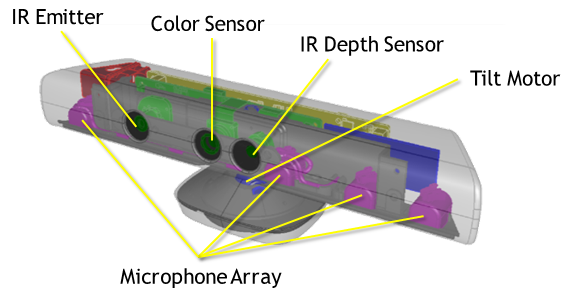
\includegraphics[width=0.8\textwidth]{img/content/kinect_interior.png}
\caption[Schematische Ansicht der Sensoren einer Kinect for Windows]{Schematische Ansicht der Sensoren einer \textit{Kinect for Windows} (Quelle: Microsoft Corp.\footnotemark[1])}
\label{fig:Schematische Ansicht der Sensoren einer Kinect for Windows}
\end{figure}

\begin{itemize}
  \item Eine RGB-Kamera mit einer Aufl\"osung von 1280x960.
  Dies erm\"oglicht eine Farbbilderfassung
  \item Ein Infrarot (IR) Emitter und ein IR Tiefensensor.
  Der Emitter emittiert infrarote Lichtstrahlen und der Tiefensensor erfasst die an den Sensor reflektierten Strahlen.
  Die reflektierten Strahlen werden in Tiefeninformation umgewandelt, in dem der Abstand zwischen Objekt und Sensor bestimmt wird.
  Dies erm\"oglicht die Erfassung von Tiefenbildern
  \item Ein \gls{Beamforming}, das vier Mikrofone zur Soundaufnahme enth\"alt. Die Anzahl der Mikrofone erm\"oglicht nicht nur die Aufzeichnung von Audiodaten,
  sondern auch die Lokalisierung der Soundquelle und die Richtung des Audiosignals
  \item Ein 3-Achsen-Beschleunigungssensor, konfiguriert f\"ur einen Bereich der zweifachen Erdbeschleunigung, um die gegenw\"artige Ausrichtung der Kinect zu bestimmen
  \item Ein Kippmotor, zur automatisierten Justierung der Sensoren
\end{itemize}

Weitere Details der technischen Spezifikation einer \textit{Kinect for Windows} sind in Tabelle~\ref{tab:Kinect - technische Spezifikation} aufgelistet:

\begin{table} [H] % \scriptsize
\begin{center}
\caption[Technische Spezifikation der Kinect for Windows]{Kinect for Windows -- technische Spezifikation \footnotemark[8]}
\label{tab:Kinect - technische Spezifikation}
\begin{tabular}{|p{5.7cm}|p{9cm}|}
\hline
\textbf{Kinect} & \textbf{Spezifikation} \\
\hline
Blickwinkel & $43\degree$ vertikales, $57\degree$ horizontales Blickfeld \\
\hline
Vertikaler Neigebereich & $\pm 27\degree$ \\
\hline
Bildwiederholrate (Farb und Tiefensignal) & 30 Bilder pro Sekunde (FPS) \\
\hline
Audioformat & 16-kHz, 24-bit mono pulse code modulation (PCM)\\
\hline
Audioeingang & Ein Vier-\gls{Beamforming} mit 24-Bit Analog-Digital-Wandler (ADC)\\
\hline
Datensignal--Tiefensensor & 640x480 16-bit, 30 Bilder pro Sekunde \\
\hline
\multirow{2}{*}{Datensignal--RGB-Kamera} & 1280x960 16-Bit, 12 Bilder pro Sekunde\\
& 640x480 16-Bit, 30 Bilder pro Sekunde \\
\hline
Tiefensensorreichweite & 0,4 -- 4 m\\
\hline
\multirow{2}{*}{
\textit{\gls{Skeletal Tracking System}}} & Erkennung von bis zu sechs Benutzern, zwei davon trackbar/verfolgbar\\
& Verfolgung von 20 Gelenken pro aktivem Nutzer\\
\hline
\end{tabular}
\end{center}
\end{table}

\footnotetext[8]{\href{http://msdn.microsoft.com/en-us/library/jj131033.aspx}{\enquote{Kinect for Windows Sensor Components and Specifications}} msdn.microsoft.com. Abgerufen Dezember 21, 2012}

\subsection{Software}
Durch die Ver\"offentlichung eines \glslink{SDK}{Software Development Kits} ist es m\"oglich, die Kinect in eigene Pogramme einzubinden und neue Anwendungsf\"alle zu bearbeiten.
Dazu hat Microsoft ebenfalls ein Handbuch ver\"offentlicht \cite{bib:kinect_hig}, das Informationen und Ratschl\"age zum Entwurf von Anwendungen liefert.
\subsubsection{Kinect for Windows SDK}
\label{subsubsec:Kinect_SDK}
% N\"otig f\"ur Steuerung der Kinect
Das \textit{Kinect for Windows SDK} steht aktuell in der Version 1.6 \footnote{\href{https://www.microsoft.com/en-us/kinectforwindows/develop/}{Downloadseite des SDK}. Microsoft.com. Abgerufen Dezember 21, 2012}
bereit. Dabei kann direkt in den Programmiersprachen C++, C\# , und Visual Basic auf einer Windows 7 Plattform entwickelt werden.
\newline
Das SDK umfasst dabei folgende Funktionen \footnote{\href{http://msdn.microsoft.com/en-us/library/hh855348.aspx}{\enquote{Kinect for Windows Programming Guide}}. msdn.microsoft.com. Abgerufen Dezember 23, 2012}:
\begin{itemize}
  \item Treiber und technische Dokumentation zur Implementierung von Anwendungen, die Kinect for Windows sensoren nutzen
  \item Referenz APIs und Dokumentation zur Programmierung von \textit{managed} und \textit{unmanaged} Code.
  Die APIs stellen mehrere Mediensignale bereit
  \item Beispiele und Best-Practice-L\"osungen
\end{itemize}
\subsubsection{Weitere Frameworks}
Da Microsoft die Nutzungsm\"oglichkeiten seines SDK hinsichtlich verwendeter Pogrammiersprache und Plattform einschr\"ankt, begannen Forscher eigene Frameworks und Treiber zur Nutzung der Kinect zu entwickeln\footnote{\href{http://hackaday.com/2010/11/11/open-source-kinect-contest-has-been-won/}{\enquote{Open Source Kinect contest has been won}}. hackaday.com. November 11, 2010. Abgerufen Dezember 21, 2012}.
PrimeSense selbst ver\"offentlichte Treiber und Middleware f\"ur die Kinect \footnote{Mitchell, Richard (Dezember 10, 2010). \href{http://www.joystiq.com/2010/12/10/primesense-releases-open-source-drivers-middleware-for-kinect/}{\enquote{PrimeSense releases open source drivers, middleware for Kinect}}. Joystiq. Abgerufen Dezember 22, 2012}, 
als das offizielle SDK noch nicht zur Verf\"ugung stand.
\newline
Das Ziel dieser Frameworks war es zu meist, Kinect-Steuerung unter Unix-Plattformen und Programmiersprachen, wie Java, nutzbar zu machen.
Ein Teil dieser Ausarbeitung ist es, ein f\"ur die Aufgabenstellung und Zielsetzung der Studienarbeit passendes Framework zu bestimmen.
\newline
Verbreitete L\"osungen, die im Kapitel~\ref{chap:Kinect} n\"aher betrachtet werden, sind:
\begin{itemize}
  \item OpenNI
  \item OpenKinect
  \item jnect
\end{itemize}

\section{Java}
% Entwicklungsumgebung \ldots
Die Anwendung, die im Rahmen dieser Arbeit entsteht, wird auf Basis der Programmiersprache Java und der Entwicklungsumgebung Eclipse erstellt.
Die Nutzung der Kinect und des Kinect SDK unterst\"utzt nativ nicht die Entwicklung auf Basis von Java, wie in Abschnitt~\ref{subsubsec:Kinect_SDK}
festgestellt wurde. Da jedoch die Expertise der Autoren dieser Arbeit im Java-Umfeld liegt, wird die Anwendung dennoch in der Programmiersprache Java umgesetzt.

\subsection{Grafische Oberfl\"ache}
% Darstellung der Anwendung, der Gesteneingabe etc.
Das \gls{GUI} ist ein wesentlicher Bestandteil der Anwendung, da hier\"uber der gesamte Informationsaustausch mit dem Nutzer der Kinect stattfindet.
Dabei wird auf verschiedene Techniken gesetzt, die im folgenden kurz beschrieben werden.
\subsubsection{Grafische Darstellung}
Die grafische Darstellung der Interaktion zwischen Akteur und Kinect ist ein wichtiger Bestandteil dieser Anwendung.
Zur Anzeige aufw\"andiger grafischer Objekte wird auf die \gls{LWJGL}\footnote{\href{http://www.lwjgl.org/}{\enquote{LWJGL Lightweight Java Game Library}} lwjgl.org. Abgerufen Januar 1, 2013} gesetzt. 
Diese Java-Bibliothek stellt eine API zum Zugriff und zur Verwendung der bekannten \gls{OpenGL}\footnote{\href{https://www.opengl.org/}{\enquote{Startseite der Bibliothek}} opengl.org. Abgerufen Januar 1, 2013} bereit.
ads;lfkj'w4kj'wrelk
\subsection{Rich client platform}
Die \gls{RCP} ist Werkzeug zur Entwicklung von unabh\"angigen Software-Komponenten, die nicht nur auf \acrshort{GUI}-Komponenten beschr\"ankt ist
\footnote{\href{http://wiki.eclipse.org/index.php/Rich_Client_Platform}{\enquote{Rich Client Platform}}. wiki.eclipse.org. Abgerufen Januar 1, 2013}.
Dabei liegt der Fokus auf Client-Applikation, worunter auch die Andwendung dieser Arbeit f\"allt.
aelkrjqw';lkjads;
\subsubsection{EMF -- GEF}

\subsection{OSGI}


\section {Roboter - Ausblick}
% offene Schnittstelle, Arbeiten f\"ur 2. Studienarbeit \ldots

\section{Mustererkennung}
% kurzer Einblick in m\"ogliche Techniken/Techologien f\"ur Gestenerkennung \ldots
	\chapter{Kinect--Framework}
\label{chap:Kinect}

\section{Microsoft Kinect SDK}
% Auflistung der Bereitgestellten Funktionen und Umfang des SDK-Toolkits
asdf
\section{Java Frameworks}
% Nutzung von Java begr\"unden etc.
adsf
\subsection{OpenNI}
% Einf\"uhrende Worte zu Framework: Initiator und Startzeitpunkt des Projekts, aktuelle Version
\subsubsection{Beschreibung}
% Beschreibung von Homepage nehmen und umschreiben und etwas ausschm\"ucken
adsf
\subsubsection{Technische Daten}
% Auflisten des Funktionsumfangs und der Details
\subsubsection{SWOT--Analyse}
% Tabellarischer Aufbau, Analyse des Frameworks, erkl\ahrende Worte und Begr\"undung

\subsection{OpenKinect}

\subsubsection{Beschreibung}

\subsubsection{Technische Daten}

\subsubsection{SWOT--Analyse}

\subsection{jnect}

\subsubsection{Beschreibung}

\subsubsection{Technische Daten}

\subsubsection{SWOT--Analyse}

\subsection{Scoring--Modell}
%Nutzwertanalyse aller drei Modelle im Vergleich

\subsection{Analyseergebnis}
adsasfd
%Resultat: jnect \ldots das beste vom besten
	\chapter{Konzeption}
\label{chap:Konzeption}

In diesem Kapitel wird kurz die Konzeption der Anwendung und der dazu geh\"origen Komponenten beleuchtet und die Restriktionen aufgelistet, die aufgrund der Vorgaben durch die genutzten Techniken und Softwarekomponenten zustande kommen.

\section{Technische Vorgaben}
% Einf\"uhrende Worte
Hierunter fallen die Abh\"angigkeiten zu der Robotertechnik, die in den weiteren Arbeiten rund um diese Ausarbeitung entstehen, die Ma\ss gaben, der Verwendung der Kinect und der Vorgaben der Software--Architektur.

\subsection{Vorgaben durch Kinect}
% Entfernung zur Kinect \ldots Maximale Nutzerzahl \ldots, nur sicher nutzbar unter windwos \ldots
Die Kinect for Windows ist ein Produkt von Microsoft, so auch die Kinect for Windows \acrshort{SDK}. Microsoft vertreibt beides mit der Vorgabe, dass diese nur unter Windows-Betriebssystemen, vorrangig Windows 7, lauff\"ahig sind, und vollst\"andig unterst\"utzt werden, sowie eine Installation des .Net Framework 4.0 auf dem System vorhanden sein muss \footnote{\href{https://www.microsoft.com/en-us/kinectforwindows/develop/}{Downloadseite des SDK}. Microsoft.com. Abgerufen Dezember 21, 2012} \footnote{\href{http://msdn.microsoft.com/en-us/library/jj131033.aspx}{\enquote{Kinect for Windows Sensor Components and Specifications}}. msdn.microsoft.com. Abgerufen Dezember 21, 2012}.

\subsection{Vorgaben durch Java---Eclipse}
\label{subsec:vorgabeJava}

\subsubsection{Vorgaben durch das jnect-Framework}
% Einschr\"ankung in Nutzung der KinectSchnittstelle \ldots entsprechende Entwurfsmuster n\"otig, nur eine Kinect \ldots
Das Framework jnect wurde bereits im Abschnitt~\ref{subsec:jnect}. Um das \gls{Framework} in der Eclipse Umgebung zu nutzen, muss lediglich das jnect-Plugin, sowie die beiden Module \begin{verbatim}org.eclipse.emf.core\end{verbatim} und \begin{verbatim}org.eclipse.emf.common\end{verbatim} des \gls{EMF}'s.

\subsubsection{Service--Architektur}
% Kurze Einf\"uhrung in OSGi und Begr\"undung
Durch die Nutzung der OSGi-Plattform und der \gls{Eclipse} \acrshort{IDE} wird f\"ur die Service-Architektur auf \gls{Equinox} gesetzt. 

\subsection{Abh\"angigkeit zu Robotertechnik}
\label{subsec:Robot}
% Nutzbare Roboter einschr\"anken - argumentieren, Schnittstelle beschreiben
Der Betrieb eines Roboters und die Verwendung innerhalb der Anwendung, die im Rahmen dieser Arbeit entsteht, ist bisher nicht entg\"ultig gekl\"ahrt, da noch keine Auswahl eines speziellen Modells getroffen wurden ist.
\newline
F\"ur die Implementierung in dieser Arbeit wurde ein hypothetisches Modell eines abstrakten Roboters angenommen, der in der Lage ist, sich in alle Richtungen eines drei dimensionalen Koordinatensystems zu bewegen. Es wird weiterhin davon ausgegangen, dass ein solcher Roboter in der Lage ist, sich in einem Kreis zu drehen und binnen weniger Sekunden anzuhalten.

\section{Fachliche Vorgaben}
% Einf\"uhrende Worte, warum buxton, warum kategorisieren \ldots
Da bereits alle technischen Abh\"angigkeiten aufgezeigt wurden, werden nun die Bedingungen aufgelistet, die eigentlicher Fokus dieser Arbeit, n\"amlich der Analyse und Vorgaben der Gestensteuerung.

\subsection{Vorgaben durch Mensch-Computer-Interaktion}
\label{subsec:MCI}
% was k\"onnen gesten, was soll geste f\"ur Schnittstelle k\"onnen etc.
Baudel und Beaudouin-Lafon~\cite{bib:baudel} beschreiben die Vorteile der Gestensteuerung gegen\"uber der, herk\"ommlicher Eingabeger\"ate. Dazu m\"ussen aber einige Voraussetzungen erf\"ullt sein. Nach Baudel und Beaudouin-Lafon, sind dies:
\begin{itemize}
\item[Handanspannung:] Eine angespannte Hand erleichtert die Wahrnehmung der Intention des Bedieners in einer Startposition eine Geste auszuf\"uhren. Endpositionen sollten hingegen frei von solch einer Anspannung sein
\item[Schnelle, aufbauende, revidierbare Aktionen:] Geschwindigkeit ist ein grundlegender Faktor in der Anwendung von Gesten, denn nur wenn Gesten einen Geschwindigkeitsvorteil bringen, werden diese auch eingesetzt. Zudem macht der Aufbau einer Geste aus kleinen Teilgesten, die Anwendung \"uberschaubarer und r\"ucknahme von Gesten bieten einen Komfortvorteil f\"ur den Nutzer
\item[Favorisiere eine einfache Nutzung:] Es muss stets ein Kompromiss zwischen einfachen und nat\"urlichen Gesten, die einfach zu lernen sind, und komplexen Gesten, die mehr Kontrolle bieten, eingegangen werden. Dabei sollte stets die einfache Nutzung bevorzugt werden
\item[Nutze Gesten, wo sinnvoll:] Obgleich Gesten klare Vorteile bieten, muss stets ber\"ucksichtigt werden, dass diese auch ihre Grenzen haben. Gesten sind bisweilen unter anderem ungeeignet, um pr\"azise Interaktionen durchzuf\"uhren. Hierf\"ur wird immer noch ein physischer Kontakt ben\"otigt (z.B., Steuerung des Cursors weiterhin per Maus)
\end{itemize}

\section{Das resultierende Konzept}
\label{subsec:Konzept}
% Benotigt wird Kreisbewegung, Bewengung in Richtung mit Richtungsanpassung, und Haltezeichen - 3 + Sprache \ldots
% Modelle zur Erkennung in separatem Kapitel
In Abschnitt~\ref{subsec:Robot} wurde bereits der hier verwendete hypothetische Roboter kurz vorgestellt. Dabei ergab sich folgende Liste an Funktionen:
\begin{itemize}
\item Kreisdrehung
\item Geradeaus fahren
\item In einem Winkel fahren
\item Anhalten
\end{itemize}
Dar\"uber hinaus kann noch das Blockieren der Gesteneingabe hinzugef\"ugt werden. Setzt man nun all diese Funktionen und M\"oglichkeiten in Gesten und Bedienungsanweisungen um, so erh\"alt man folgende Anweisungen:
\begin{itemize}
\item Kreisbewegung
\item Vorw\"artsbewegung
\item Haltesignal
\item Blockieren--Entriegeln
\end{itemize}
Diese Liste wird in Kapitel~\ref{chap:Gesten} verwendet, um die in der Anwendung eingesetzten Gesten zu modellieren.
\newline
Die aus der Liste entworfenen Sprachbefehle werden in Kapitel~\ref{chap:Sprachbefehle} erl\"autert.
	�e�eUے��w��Q��PO�
�skƈ�7)"e�F����j�3�o|^o0��L7ͩq�o�v�C)�K�V_f�k�{Z�ً@J�
�\��`���gq����v�Lf4aϵ��}F)�ݧ֒l��J�`�ʀ����Lv�M��/�GtD%!N���<#���}��I
̳�%�={��Dr�LK kmZHq=dԥ�lT�/N���ޜ9���U�+����9�r�dz ��֒������K@���ԓ�Z���D����Q���K]0*6�ƥ�@����EPrR�����1s����,īI;�(WM}#Ś-n��M`(N��)��Z�f*4�b�lڳ����!�f�8W�nB��vI�@��Fa�c]�9�/כ��kاQ6hX�q�M6:�����S�ラo���һlP"�>f�����Bb��O�@��YNU5ۧ@� d���p`A���pn�>�R*�Vѽc�J�$���E���OV5��SΟ�)Ӽ��y����P�I��B�SS
jN�_=�{q��b�SV�?u7��Zz�
�������0B��n��N��ݱ��.$���(B��9���m��qK��g�(�eaL�8H�����ғ�L�i�}nD�n0#���b��N_�w��ɀM|�P��RR�?��PxA��H"�����0�Ox��MT�?f_�tu4�<h�\hPV_�>ܹ� /����O��J�o�VZ%źc}iE{����=�n�uk����;�hߖ�T��ވ+$�##q�X�v���m��r�-t��7�P>*X~��$]�뿂���>u�i][�7Ń���I	.����be��y��0��ڙ1��d���J0#����6��O8/ܤ��~׆hD��{�Ձ���z����R#j�0�.&[�o�DR�������X�O���D�����j2���5K-���3�܊�Qk�
[xo�B�&�!�P�tE�����a:v�Ot/U�8�+lA����]ae������G�aR�'�Ee�R�U&��g�4aM�"���z�UB��.PC��+ߞ������S��!7�)��G��l1IW�ǝ8r	�c��}�d��E�I?�L`k��Lq��)GswmlT�T��da��aʴ�3�E�Cb��׾J���ߐ���Ң"��)��H�0�T��Y�|n&uZxVh �k���G�����~,�P][���(���� �}�[��Kh��^�A���<���O!��;Hͥ!{`���~��6��}7�c�C��@��s��5WH�^YDuҿf�	�@<��X�c)�s	��.�r����j�D9��	�ӨU	�*
*�m��^�)��C끬������	�7&?d�?�ɬ�P	��M��ǔh�V߀&�'��5Ek��B8�;Q�ںӃ^lb�:��<h;w�XV$`:
��fXZj|����P�ǭ��A���c�YÐ�"#���|+�kR�!�1I86:|#�o�`]��
��6�������E��9xg>#�{U��G�Ɨ�g������q
.to�I�Zg���~��_A��_3c0�/r):�D�I[��M:�W�t��&۩�à˴rz�n6ע�^�=�N�C�!�<�x���Os�2��4�I��,Q_m]�߅[�j�P1�P��^[��L���SU��}�x G�م��ʛ�ΠϴW
��"���t�lksa!�4��Gu�����l?Q�?v�4fT�k�����]Vfʨ�Ţ�!�*��e�A��/3�u�1Qx�J�<���e��coFt��偊��Ǜ�-��\�������?�!�)H�m&b�_��CcELvw��)����Y��!�zPL���8�YTA�1G�����d�9�
�S|A0aK�z�Nn�d���e;t�|�3l��4����l��c��껄T#F�<g�E
h*7Z@���졎�v��c�v��	����3��q�T<PG�G=Pf�}�v��H���֢�����`+����k�1䱾�����ˡ1�!�@/�zSŠ�Z��EgӜc���b�)�[RT'4����y7A�8�noZ���5���-<�cZ#��3�l~vǒ�I�1�ZN��S��0%]rlk��1���h�آ��yt)�V`OC{]����ʺ<=&m�K2]%��C �B��I+�xs]�e��� m6f`k	���'�r[9u�!��=͹�5��v�L&6�����DH嚣XVň������Z�έ��E�����7�r=?U�>�i��N���)O�VJRg��)��o�
��N�Z����8/��ϲwm;>?�[����s������y�Y���}����kc^$g�ft�[��Bl��0�y��a��ޚc��ث���W=[�Nw�<��5���NV�\d5M�+��#�M�����5e'Pyn���f��O�F$�qgN�簽Ϭ�Hm�ay�^��(�P�$mr��ﲵ���p����3���	:�t
��]�56�0�~N��`����{�
�G���@�I�U�j���4��MN-��(��K܇G��L��(�<�6�O����[ܠ��t�d�T�������_�VqT��p�t4���P�d$|���L����#�Y�h��ږ9�Ԝ��l�ӱ��J�ٍ�8�vE�s��p
=���X[��(����ޙ�j|�oGZ`zyD�.c|(0EL�L��BG�3�j�J�TF�Z�S�"�lJ0�YTM}�:�����Y��cx
�;����6�7���uN��w��Uo����y(��e�OhjdP�g�@��[��ӓ@䲪4�9����_�TY��V�_�2�������D�|��Bu�;&h�f>Y!~�g�f�����z�W��&���	�ee
�u'����hd�N(2�m���T�~�oڣ����2
�b��DM�:�|���b��ޡ���?�(���
dH��@,�1@j0��M��2䋜_���7j���$$�I]��p�e�rz��
��`�2O�O�iChL�&d�F�#�]��`�lD�����XUE�P�R�׳���j��XaI~���[JCc�	�n��XJ��v9�2!�]��`�Ƅ��u\�J)�2N8���N�����5}��9��fL/������߶��ѷ�`)?j���������&��k-Jjn�q#��|TcU�DB;e1�����ԝȏ¶w��g�5��^�~���FK�O����c�Ž��T`x%}:���4��qI�@Vl�O�����%��8���t
��‚~jprZg�4����e�7��y������K���ZW$��A=����@��g�G_���[����R=���$J�kQ��PiK�A}!	�/�Gw�Kzt�n�)�:�as#�L�[(�D��H��&p�@���\<DIv��i�����\��YG�1���=2��!���QW�ޮ�;�+�����>�};�'�s�d�S�kK�4�Q>D|j�NV��'T��x�َѠM�������8�o:N�$;���z�Ԋ;Yy
k�h�2jR�*FDC���9��/uE5������
�<�;u��w�΄��B����c��N*���(u��g'kc�߸�r3v3�Z�*�1�1��+H��Q՜XdD0�(%eie���n*�,Y1��d��gb�+�4|�ۢ�4�P5�,�{so�Al��a��V�!�"����h{���xң�L:ik]$9B�J?g����ЩƓ�4���)��+�^�骨����;�I-�#jh�fEY�5�T�_9������9�;:{�!h͑�h�a2BNe47��q�n�qG���nsW}8��- �#f�h�7���8�d2�}#�@O��MB��{��J�Na��8������(Փ=����o&��cz� �Rз���D�OZ�A�k'܀�L1Z�Vb�����΍3�竮Q5��ԉ=`��}a�֛2���0�vB�?���ȉ_=�5��}�?x�xZ��^��bI���<�ݠ��(��:�߳��:��)�Lr�a>*4���d�٧4�̓���|�����+�<�J��	_gv:�
E���^�U�I��Z����<ȵ?k�+�F��b��1e��
JU;�-LlQ��'=)��`�|3�[`P��!����TJc\�_I��v�5nI��;�spێ[\0�J[�9������in0��Dd@!wc�;���P��;zZV�°��sur�@�W��Ũ~�֛H������O�H�SW���j�`��Mj�� ���� ��t�
.�+Wy]J�4?xJ��R��?>)1�w.HR�Fh �ة�Er��*Y���Ԑ�p6�a<�3H�b���3�x�����v>1X��͹�cs\�� ��5x�]=e(����u�S*����iN�;U�^��&Pf�D�f�K�����7�:!�U7g�.m�����3F�)��EpR�5�b۱
��i?~�EQ-�7?H�)�@��"�AW��^R�0D�u�Ljl�߷T�G�5��������S{���/CŒ��dd�<m�O��"}�8����F�\qR�7����?Y�m��1�S�hr��A��;�����UQ�C>���#���>��O{��E��;���\A�%�
��9Z�-t{��T5ɠ_�mv@z
ީ��Uג�"ݗg�j�<G��!m5DF4��6K7�V�2��{�ˎBp�{\�&�E��+R֠X�l����9(�X�`��:��!�|z���vI�iR�G����A��?f�0-L8}�E^�i���2Jx���N�f��!�X繄������&G{q�J�[�ɵ@eG�J�@y��Ƞ=�S�
��.����|�_6����{݃�{��7���0�]:V��ЍV��y|s
f�V�N�Hi9��6U�+�!�\U�`�n���P
�v��gw*��oV;�ʯ���b�8�����u&�<�J��sG[�9^=�ީ�/Zt��E�q�k����L����]
�~'��@ZFO����UӞ�6,���2��w{�i/�NA]2�έ��Y���X�تQ�V�Gf��$�kr��d�����9DD����?�d�*�yp��D��N/�Pˮ��1����*�xK.3�O�$k ����*A�f�����O��b�ytml�w�^W,N#[��oϐ����'I�u����JA��(��r\!u�>#�[*DPp��]��G�϶#?hM/�ZT���I���e�ٖ���y3x9���=����%!
����iL��dlAA�e���J��>�P�S�\?��Zsp�r��9
�{%�)]JmHJ�~�J1��]�Ϸ���+M�NMk�����zA6N�1TR���WR�E�8�6���
U��0�b�����-��C�7g�T~��ˬV�}T�*p��{X�H���9=_�붒�x�:���܂�o�x!M
c~Ā>� l;�j8{~(b!�eުoK��QvzS';����BHw�e=��T8��>aF
4�/?�"�R�e���T��_�r3:�OM�xڧp����c�����43�}M|�~,1�	��;Yɻ�%���5�
5ɡ�˭�����j�L6��>�E��l��e�:&}:S3Yz3�ud�T�xz��}9'�*tc�qu|�Q��?��ޟ��v%�
�Oo�YIkYJ�W����M�f������w�Y��?ji��.l����ϒk���5n�+���8@�p����1�B����n��(D �MF	�TH�A��B��x�.���d�w�G�!�hkD�D��F���ק�������'s��Zlv
q O�ugc;L%*����独j1��b	\�I�L��ݩ����3%;}��]�K!�1�{VJ�:%�q��(��[���.��jH���7�r݃�em^�vs���~�q��-up����F��Yǎ�)�:WkQ�<[��{ܚ�F���G��2	л$���A#Uy#���[D�p�>�:G���[���(����:�5?]q��pY���(��^����6m�Kc�$J�]�����b�$yF37����cg��5��T���g���ȟK�/|�ɪ�pS"��0��G�"�Ъ>��VPa��\èXC�.(�ɫ�����G%zpbY�@D���޳�S��%��09W֘�BJ�´�������y�NFN��թ)M�y8�/�D����-����kO�%8>�q^�Z��vbo'��;���ua�IB�����'Ճ�=H�vYȑ�.��=щIw�w�q��� ���jT�rޤL����`ߠi��uY�fLO������W�:��x�*�q�'����v���eQ�Y�\J�Q�EXE��V�T���I�;sO
3d=^����\X�]����:;&������JYJ��}`�
=+�S4!F�
���y�횕����{ab��Ul��)�l����͞�ԇ;U}���?kR�{P�yԔpRg�xGH�%�z	�r
�^�r�p�d����Q���.|��wt�sHҙ����劯��ԡ�N9bsh���\I�B��"�*���Vu��MI	>z0[U�BI�lؘ���?��0��S�ǟR�q��tN:�I��B-@L~pƯ��
�m�pi�ndz��Y+����#�0~R31���VҜ�/i�7��Hw�g��/[�ꃺ���
&OZi<#7��O�_mQ�j����R���]���c�x��86��B1V��T-���g��ʯDs��#������3x�czgx��<1�\}��ߨV3-R��Zd@��0SZ�8\T��k�|
�h�+�@\g�8�ſxJ��H+�l��L4뢤Ŵ�I��6-|3e������^�5�8�͘�
��)
h�,Zx��H򰬐�]r�rLȨ��.�i�lf�<��T��X��k������a ��%���#��`�~�*���y����|����N6�Q��2���ϱdv&���2Y=��>�ke�G�.U�?��B6ˍ���;�ޏ��U�WZVy%E��J�ɰ��PO�h�O��!�:�@r���\�����ދ���P(��;��l]Y���V���F���x�,����x{ cȇ@qy�b�tsw*�L�����?P_�_ف�����	Op�7�cI��MI�[�~�l�\JK��+D��w3�o~���7���8y�'��*�Y[����Ev��⫚Y��h�8��!��)��r�(�Pj,LPD�U��/������[w3;p(Q��^�ݱ��'�Os��!s�_&�=k�zO���EĞ��l���c�֬�$���e�~�Y��>P�5���,��rR�{\�'N���qk�z�Rt����r�u���ݏ�a���k�3Шf��I7#�#�����2��㤪�f�k׿�b]IѶa:3D*�#4��w:^�J@�jx��OT�u��Or
�5?\$9aIE�#���r�/k��l��G;��+�����(�+�}��G���E�0+�����
M �Px�e����~KU�t��'�p%�hixm%�+��\C������
�b#P�5�L�W��N�c\V�6
Z�DN?�E�a����8���7��x�iͷ���v�1��~�Z�a%ƴ��KT���f&���e�3��;�ف����{KM�#��?�j���N�Ū�GJ��f:y�?��r��sN�b��Ri}��GϏ)��ʵ�Z��Y���j����-FRw������FH�߾D��M��h��nd>Y<��Q�y��s�ǥ�����v88�]򉅼�Em�"��~T-�
�Ӗ�:��Γ4�)ɥ8���T��E����`3�w��q�Z� ��e.���pR)bZm�8�]���(�̙�ii�]��������۩�2�j���p�ֿ�#
x�|[�?���8�F���j:@2ܫI����C����V4��݊K�}2����L�ieN��T��M)vV3PK]E�)@���;K%��Vya7WF�LEK��|�$����"�d�>"uz��U}^񄓐���S��b�ǘ�V�©�I���I��f�y	���Jq(L��;�w�;�$�!������(�`X��bq]M��u�k��z�)}V]X�Ŧ����:���*�`�&4�"��#�ծ�NYVt��W��y�[�f`#�6�m�a��@�B�"!���,g�B�ۭ�k
���:hu���U<��7�L�����9�$SX�֌�rs%|��a�ջ��*-�=�Pb�w��3��pHE��f��z���,��tԞ�Y&��v���"C��}��:5�	s��b�(Г�
D���T��l���'��Z�;7�
(�[���j�2[-9�k��j7�X~7�DX�ؔW�N"n��,�Q��I��զ��?�qj�=?@�>H��DVgڒ�!���%���V�=6�G�XX�����ޅ�;3����g���ڭ��F�oC6���xnu[&� ��G'ދi
e��L�m,
2�!z��ķ�~_��w���5���&�=��f��-��%h�dRu����t-XyUa�d��Qe8�/�|�.U���+���v�r$ȍj�o�8q�j|�?z��yqUD�e^kg1NI�G�`�|k����zO٪�"rz	�
w�~�3�߆�'��������m�Oʹ�龝%�p�@ٛ�H���s-�-ݽ2���#�F�T}�D��~v��AA��)ruth��"@>��ݠ�P�x��K����-Q�gȆ�|%2��
pg���7��}!� �� �7������i4h�N�4l�pY$Q��t7he���Kq��59KD��h}�#e�_�;��޾�ʍ���"�!}.:�lëf���t�K�+Sq/^�=ˆU�&��\���~;-gY�:ly�v�w��ɇ�7�e�\F������b����m�iaFc�/�E�����2
V�	���g��fp����mSuK�M	��2rT����f�0�:)Y�������"��]纅�V+i�iP/*%o7����X���p��V�76yЖ�:�•*��,*�L�u:}���ۇ����AH��-���A�.�O��1�QW"���Qj�8F���鈨XPyK�$+��'%RL������ItCd��`8_�#�C�we��5�NL։g��D�[��je�讓�J;ίlvv�%�](Px?k�ue���3D�m�m0I� {q��ޔW�
D�~�N[�Q�Yt]���VcT��`�B�ݎ�����I=�܉�4�G���;��`��s�Rf_Z%1�Kwɼ�$Li���Fjo�M'0׺��`��UX	R�`}`I�B��1�S<z}n�Uy ?�G΂>nϝ�^3�Nr������_�E�E��|�R4�2ӔA�2�
�9�&,m;�îZw��|�I����?�~��*��g-
!��A7��TS-���d�@�\�Aa6~_&������8�i���*���9D!|}@�Sĩ��&P��Y�=<�o(}���~�@R�q�3��Z}�|Ę�YIoX�>�r���k3y�"EҼ�7� ��p-����G,��%���Z▕j�!�k���j�nJ^�j&�mb+�=���H�/�*8W6_1X�<�s����$i��^8@����O�t�O�3��8��Gˤ�cL��R2".w榻��;���.�3�^/h=�`�UB|�NC}� ��ޖ�P�-,h���>L
�C@�+0�����4�
P�rJs�J���
�z+�Ʀ�s5�4�N��
�3��_C!Vw����p���S��&�LjۻN���F�vT;]M�o|m_��n���xo�ӿ�
�����
	��~��i������
q۴C9��68�ϥɇ���#�.����9z�}/
�r�C�yښ�?>^6?��A�t9���%�Ĕ�d�Q�q+���I(�������[��5V��/b胘dη���M5�C�O(�ݗ�9ľ��z8�Esά��J[ŒeHRg�n��!���1�;����,�L+͔?�g%�e4q��r��d�hi����GSv�s��m��vB+���Z�|�Č1Hiɚ���߃�
�y$�1@w(�$�+��������j�I��׻�2�,��x������g1��:Y�GYu�EMW�ʬ�
C��T��X=�ȸ�F.g=A�kx8(��Rb��B�'���6�se��
�2,ZU"�6�%�B�t$�����we4¨�V��	 ��E��3�lʝڽΔF1-�J���V��������'���:'�X^�d,�P��EYBp�pT����$L-�)ix�C��k��'���<�UX���Ȭ��Lм��&밾���|�@���/4�B�<�c���v27�S-l��ە�\�g�W�g��{�V�F����O�e8~��E���,u: �J�q���c[g�R�y���Oz��?�[�3_[��y��y��ȵ�\F�}:2 �
��C�88��`F���:J}3(���D�Ԧݒ��3�=���]4;	��;������|��da�z�LS���d>�F
GK�J\�Ǐ�/H�_R�x��	���z��U���uʧ$�R+o�қ�i�{�n�/&��l����bwbQ��n�(A���+"���[}�3�����)ʘ7,�
���4�Rh�9�Y�#��$Q
X(��1{$!�=[+�Rz��T4�ϒ�x��`��@9U��Q)fB�S�$e��@k.�8���o�������I��������~@L���w�h1�7�.��`��b$�/J�ip��ڸ_���ewE�y|���D8��Bz����^8V1n:r
K���蹤�Z#z�n������;��u���(�	����H�ϊge7�c�A+[4�'���9?V����KOv<���@�M�;�ʱY�A��[�<i��f]��\#�w#����9?�S[�籊v|0�%�U@��?W��߲���Qr��w�Ye�Ca�@����ײ`�O)���h��G/�t���@&�
��~��k0��YF�c��R/ Y�gq���^
ak��D��0�y92��u	������rLE�VaM��&���2t+�~�d.)���H\����mP�e�	)�p�X	ʑ��~�O�\:H�̱��)�9��Z��ǫ{c�AYu+݂|$�0���P��R�@�t0(�>p��8���X�d�wu]�;�
�i���81�‡���x�G�V���)�O�yМ��4�p>��C�K/�2��1QDDAF"�+e��o3�������]Xz����V��b��ƣ��J��&d�ouf�7�٠(�*(��e�R�[��GE����.!GI�8����l����E>(BxKk�#�F2�]au����'�ߝN��j��f�{��i��(F��j�@���k.�8��ș"c,��s'b���j++�� �ޓ�dȝ�֚���$�=}SvL�a}[p��%Eՠ@1�!�e��
<��TH}�)�e��ǜ-�s
j��u����bw/C
	\chapter{Gesten}
\label{chap:Gesten}
% Einf\"uhrung
Gestik spiegelt einen wesentlichen Teil unseres Alltags dar. Als Teil der nonverbalen Kommunikation dienen sie zum Ausdruck von Emotionen, zur \"Ubermittlung von Einstellungen, zur Darstellung von Pers\"onlichkeitseigenschaften oder Modulation einer verbalen Nachricht, so Archer und Akert~\cite{bib:archer}. 
\newline
Nachdem bereits die wissenschaftliche Definition einer Gesten nach Kurtenbach und Hulteen in Kapitel~\ref{chap:Einleitung} aufgef\"uhrt wurde und einf\"uhrende Beispiele erl\"autert wurden, werden hier Gesten tiefgehender betrachtet.

\section{Kategorisierung}
Gesten k\"onnen isoliert, oder im Zusammenhang mit einem externen Einfluss oder Objekt existieren. Ein bekanntes Beispiel f\"ur isolierte oder auch freigestellte Gesten, ist die Zeichensprache. In Bezug auf Objekte gibt es eine gro\ss e Bandbreite an m\"oglichen Gesten.
\newline
Daher wurden Gesten in Klassen eingeteilt, um diese besser unterscheiden zu k\"onnen. Die Klassifikation nach Cadoz~\cite{bib:cadoz}, die Gesten nach deren Funktion gruppiert, defniniert drei Typen:
\begin{itemize}
\item \textit{\glslink{Semiotik}{semiotisch}}: Diejenigen Gesten, die aussagekr\"aftige Informationen kommunizieren
\item \textit{\glslink{Ergo}{ergodisch}}: Diejenigen Gesten, die genutzt werden, um das reale Umfeld zu manipulieren und Gegenst\"ande  zu erstellen
\item \textit{\glslink{Epistemik}{epistemisch}}: Diejenigen Gesten, die genutzt werden, um von der Umwelt durch taktile und haptische Erkundung zu lernen
\end{itemize}
Dar\"uber hinaus werden diese Klassen weiter unterteilt. Das Augenmerk dieser Arbeit liegt auf den semiotischen Gesten. Innerhalb dieser Kategorie liefert Mulder~\cite{bib:Mulder} eine weitere Sammlung an verschiedenen Klassifikationen.
\newline
Da der Fokus dieser Arbeit auf der \gls{MCI} liegt, werden vorrangig sogenannte \textit{empty handed} semiotische Gesten betrachtet. Diese k\"onnen entsprechend ihrer Funktionalit\"at weiter unterteilt werden. Rime und Schiaratura~\cite{bib:rime} beschreiben folgende Taxonomie:
\begin{itemize}
\item \textit{symbolische Gesten}: Dabei handelt es sich um Gesten, die innerhalb eines bestimmten Kulturkreises, eine allgemeing\"ultige Bedeutung erlangt haben. Das \enquote{Daumen Hoch}-Zeichen, w\"ahre ein solches Beispiel
\item \textit{\glslink{Deixis}{deiktische} Gesten}: Unter dieser Kategorie fallen Gesten des Zeigens oder der Richtungsweisung. Diese stehen meist in einem Kontext, wie \enquote{Lege das hier hin}
\item \textit{\glslink{Ikoni}{ikonische} Gesten}: Darunter fallen Gesten, die Informationen \"uber Form, Gestalt und Auspr\"agung eines bestimmten Gegenstandes oder einer Handlung
\item \textit{\glslink{Panto}{pantomimische} Gesten}: Dies sind Gesten, die typischer Weise die Nutzung eines nichtgegenw\"artigen Gegenstandes oder Werkzeugs wiederspiegeln. W\"ahrend der Mimik einer Aktion wird dabei eine pantomimische Geste gemacht
\end{itemize}
Baudel und Beaudouin-Lafon~\cite{bib:baudel} zeigen einige Vorteile der Nutzung von symbolischen Gesten zur Interaktion auf:
\begin{itemize}
\item \textit{Nat\"urliche Interaktion}: Gesten sind eine selbstverst\"andliche Form der Interaktion und einfach zu verwenden
\item \textit{Knapp und Ausdrucksstark}: Eine Geste \"ubermittelt genug Information, um Befehl und Paramter zu liefern
\item \textit{Direkte Interaktion}: Einzelne K\"orperteile, insbesondere die Hand, als Eingabeger\"ate machen weitere Signalgeber zwischen Eingabe und Empf\"anger obsolet
\end{itemize}
Nat\"urlich bergen diese auch Nachteile. So k\"onnen symbolische Gesten auf Dauer anstrengend und aufw\"anding werden. Ein Nutzer ben\"otigt in aller Regel Training und ein detailiertes Wissen \"uber Anwendung und Funktion der Gesten, bevor er in der Lage ist, die Anwendung mittels symbolischen Gesten zu bedienen. Je weiter die Anzahl der Gesten und deren Komplexit\"at steigt, desto schwieriger wird es, sich an bestimmte Gesten zu erinnern.
\newline
Weiter stellt sich ein Segmentierungsproblem, dahingehend, dass eine Bewegungsdetektion in aller Regel, den gesamten Verlauf einer Handbewegung, oder die eines anderen K\"orperteils erfasst und die eigentliche Geste nur einen Ausschnitt dieses kontinuierlichen Signalstroms darstellt.
\newline
Es ist daher wichtig, Gesten, die in einer Anwendung verwendet werden sollen, so zu modellieren, dass sie einfach auszuf\"uhren sind, eine angemessene Unterscheidung zwischen diversen Gesten vorhanden ist und diese sich m\"oglichst nahe an nat\"urlichen Bewegungen orientieren.

% jede Geste genau beschreiben - grafik dazu \ldots konzept \ldots realbild von kinect
% hmm modell, genaue beschreibung, stati, \"ubergangsmatrix, zahlen zahlen zahlen
% verkn\"upfung mit aktion f\"ur roboter
\section{Gesten in der Anwendung}

Nachdem bereits in Abschnitt~\ref{subsec:Analyse} die Anforderungen an Gesten ausgef\"uhrt wurden, werden hier die daraus entwickelten Gesten aufgef'\"uhrt. Dabei werden alle grundlegenden Vorgaben f\"ur ein \gls{MCI} aus Abschnitt~\ref{subsec:MCI} ber\"ucksichtigt und die zu entwerfenden Gesten auf Basis der oben beschriebenen Kategorie der \glslink{Semiotik}{semiotischen} Gesten modelliert.

\subsection{Kreisbewegung}
Ein abstrakter Roboter, ist in aller Regel in der Lage, sich im Stand vollst\"andig um seine eigene Achse zu drehen. Dies ist eine hilfreiche Funktion zur Steuerung eines solchen Ger\"ats. Betrachtet man diese Drehung, so findet im Grunde eine Kreisbewegung statt. Um eine intuitive Assoziation zwischen dieser Drehung und der daf\"ur zu verwendeten Geste herzustellen, wird zur Durchf\"uhrung dieser Geste, eine Kreisbewegung verlangt. Das hei\ss t bildlich gesprochen, dass der Bediener mit seinen H\"anden einen Kreis in die Luft zeichnen muss, um die Geste auszuf\"uhren.
\newline
Die Ausf\"uhrung dieser Bewegung ist intuitiv und ohne nennenswerten Trainingsaufwand anwendbar.

\subsubsection{Fachliche Aspekte}
Die Kreisbewegung ist eine \glslink{Ikoni}{ikonische} Geste, da sie die Form eines Kreises wiedergibt. 

\subsubsection{Technische Aspekte}


\begin{figure}[htb]
\centering
\begin{tikzpicture}[
    scale=4,
    axis/.style={very thick, ->, >=stealth'},
    every node/.style={color=black},
    auto,
    ]
    % axis
    \draw[axis] (-1,0)  -- (1.1,0) node(xline)[right]
        {$x$};
    \draw[axis] (-0.5,-0.5) -- (0.5,0.5) node(zline)[above] {$z$};
    % Lines
    \draw[axis] (0,-1) -- (0,1.1) node(yline)[above] {$y$};
    % Lines

\filldraw[fill=gray!5,fill opacity=0.8] (0,0) circle (0.8);

\fill  (0,0.8) circle (.4pt) node[above right]{$S_1$};
\fill  (0.62,0.5) circle (.4pt) node[above right] {$S_2$};
\fill  (0.8,0) circle (.4pt) node[above right] {$S_3$};
\fill  (0.62,-0.5) circle (.4pt) node[ right] {$S_4$};
\fill  (0,-0.8) circle (.4pt) node[above right] {$S_5$};
\fill  (-0.5,-0.62) circle (.4pt) node[above right] {$S_6$};
\fill  (-0.8,0) circle (.4pt) node[above right] {$S_7$};
\fill  (-0.62,0.5) circle (.4pt) node[right] {$S_8$};

\draw [->, thick] (0.05, 0.95) arc (90:-265:0.95);
\end{tikzpicture}
\caption[Abstrakte Darstellung einer Kreisbewegung im Koordinatensystem inklusiver ihrer 8 Zustandspunkte]{Abstrakte Darstellung einer Kreisbewegung im Koordinatensystem inklusiver ihrer 8 Zustandspunkte}
\label{fig:Circle_ideal}
\end{figure}

In einem \acrshort{HMM} wird diese Bewegung durch acht Zust\"ande modelliert. Abbildung~\ref{fig:Circle_ideal} zeigt ein ideales Bild dieser Geste mit ihren acht Zust\"anden.

\begin{figure}[htb]
\centering
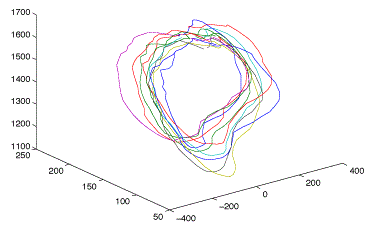
\includegraphics[width=0.5\textwidth]{img/gesture/gesture_circle_real.png}
\caption[Darstellung von Kreisbewegungen im Koordinatensystem die aus realen Trainingsdaten stammen]{Darstellung von Kreisbewegungen im Koordinatensystem die aus realen Trainingsdaten stammen\protect{\footnotemark[1]}}
\label{fig:Circle_reall}
\end{figure}

Diese acht Zust\"ande bilden ein Mittelma\ss dar, um auf der einen Seite kein unterdimensioniertes \gls{HMM} aufzustellen, auf der anderen Seite, aber gen\"ugend Spielraum f\"ur die Akzeptanz von Kreisbewegungen einer etwas ungenauen Form zuzulassen. Abbildung~\ref{fig:Circle_real} zeigt mehrere solcher Kreise, die aus Trainingsdaten ermittelt worden sind.

\footnotetext[1]{Quelle:~\href{http://www.creativedistraction.com/demos/gesture-recognition-kinect-with-hidden-markov-models-hmms/}{\enquote{How to Do Gesture Recognition With Kinect Using Hidden Markov Models (HMMs)}}. creativedistraction.com. Abgerufen Januar 14, 2013}

Die \"Ubergangsmatrix $A$, f\"ur die Geste einer Kreisbewegung wird definiert, als
\begin{equation}
\mathbf{A} = 
\begin{pmatrix}
a_{11} & a_{12} & 0 & 0 & 0 & 0 & 0 & 0 \\
0 & a_{22} & a_{23} & 0 & 0 & 0 & 0 & 0 \\
0 & 0 & a_{33} & a_{34} & 0 & 0 & 0 & 0 \\
0 & 0 & 0 & a_{44} & a_{45} & 0 & 0 & 0 \\
0 & 0 & 0 & 0 & a_{55} & a_{56} & 0 & 0 \\
0 & 0 & 0 & 0 & 0 & a_{66} & a_{67} & 0 \\
0 & 0 & 0 & 0 & 0 & 0 & a_{77} & a_{78} \\
0 & 0 & 0 & 0 & 0 & 0 & 0 & a_{88} \\
\end{pmatrix} \, .
\end{equation}

Dabei ist der \"Ubergangskoeffizient $a_{88}$ gleich $1$. Weiter wird zur Initialisierung f\"ur die weiteren Indizes $i, j$ auf der Hauptiagonalen und der rechten Nebendiagonalen, $a_{ij} = 0,5$ gesetzt. In Trainingsdurchl\"aufen m\"ussen diese Wahrscheinlichkeiten eventuell vereinzelt angepasst werden.

\subsection{Vorw\"artsbewegung}

Die Fortbewegung und die grundlegende Bewegung nach vorne ist die Voraussetzung, damit ein Roboter \"uberhaupt bedient werden kann. Doch diese Bewegung als Befehl zu \"ubergeben, ist wiederum nicht so simpel. Es mehrere M\"oglichkeiten, eine Geste hierf\"ur umzusetzen. Die L\"osung, die hier verwendet wird, basiert auf der Idee der Richtungsanweisung. Das hei\ss t, dem Roboter wird die Anweisung gegeben, sich geradeaus nach vorne zu bewegen.
\newline
Hierbei wird wird ausgehend von der Hand modelliert. Dabei wird ausgehend, von einer K\"orperhaltung, in der die \"uberwachte Hand in N\"ahe des K\"opers auf H\"ohe des Schulterblatts liegt, der Ausgangspunkt festgelegt. Die Aus\"uhrung und Verst\"andlichkeit dieser Geste ist relativ einfach, da sie einfach eine fallende Handbewegung dargestellt. Abbildung~\ref{fig:Forward_ideal} zeigt eine schematische Darstellung mit vier Zust\"anden.

\subsubsection{Fachliche Aspekte}

Die Vorw\"artsbewegung ist eine \glslink{Deixis}{deiktische} Geste, da sie eine Richtungsanweisung wiedergibt. 

\subsubsection{Technische Aspekte}

In einem \acrshort{HMM} wird diese Bewegung durch vier Zust\"ande modelliert. Diese vier Zust\"ande bilden \"ahnlich, wie bei der Kreisbewegung, ein Mittelma\ss dar, ausreichend Spielraum f\"ur die Akzeptanz einer Vorw\"artsbewegung einer etwas ungenauen Form zu besitzen.

\begin{figure}[htb]
\centering
\begin{tikzpicture}[
    scale=4,
    axis/.style={very thick, ->, >=stealth'},
    ]
    % axis
    \draw[axis] (-0.1,0)  -- (1.1,0) node(xline)[right]
        {$x$};
    \draw[axis] (-0.1,-0.1) -- (0.5,0.5) node(zline)[below right] {$z$};
    % Lines
    \draw[axis] (0,-0.1) -- (0,1.1) node(yline)[above] {$y$};
    % Lines

\filldraw[fill=gray!20, fill opacity=0.8] (0,0.8) .. controls (0.1,0.8) and (0.35,0.66) .. (0.48,0.48);
\filldraw[fill=gray!20, draw=gray!20, fill opacity=0.8, draw opacity = 0.8](0,0.8) -- (0.48,0.48) -- ( 0,0);
 \draw  (0.1,0.1) arc (90:10:0.1)  ;
\fill (0.11,0.048) circle (.2pt) ;

 \node[] at (65:0.3)  {$\alpha$};

\fill  (0,0.8) circle (.4pt) node[above right] (a) {$S_1$};
\fill  (0.15,0.74) circle (.4pt) node[above right] {$S_2$};
\fill  (0.35,0.61) circle (.4pt) node[above right] {$S_3$};
\fill  (0.48,0.48) circle (.4pt) node[above right] {$S_4$}
 edge[pil,<-, bend right=60] (a);
\end{tikzpicture}
\caption[Abstrakte Darstellung einer Vorw\"artsbewegung im Koordinatensystem inklusiver ihrer 4 Zustandspunkte]{Abstrakte Darstellung einer  Vorw\"artsbewegung im Koordinatensystem inklusiver ihrer 4 Zustandspunkte}
\label{fig:Foward_ideal}
\end{figure}

Die \"Ubergangsmatrix $A$, f\"ur diese Geste wird definiert, als
\begin{equation}
\mathbf{A} = 
\begin{pmatrix}
a_{11} & a_{12} & 0 & 0\\
0 & a_{22} & a_{23} & 0 \\
0 & 0 & a_{33} & a_{34}\\
0 & 0 & 0 & a_{44} \\
\end{pmatrix} \, .
\end{equation}
Die selben Bedinungen f\"ur die \"Ubergangskoeffizienten gelten f\"ur die Vorw\"artsbewegung, als f\"ur die Kreisbewegung definiert wurden. 
\newline
Der\"Ubergangskoeffizient $a_{44}$ ist gleich $1$. Weiter wird zur Initialisierung f\"ur die weiteren Indizes $i, j$ auf der Hauptiagonalen und der rechten Nebendiagonalen, $a_{ij} = 0,5$ gesetzt. In Trainingsdurchl\"aufen m\"ussen diese Wahrscheinlichkeiten eventuell vereinzelt angepasst werden.

\subsection{Erweiterte Vorw\"artsbewegung}
\label{subsec:gesture-extforward}

\begin{figure}[htb]
    \centering
    \subfigure[Darstellung der gesamten erweiterten Vorw\"artsbewegung mit 6 Zust\"anden]
    {
\begin{tikzpicture}[
    scale=4,
    axis/.style={very thick, ->, >=stealth'},
    every node/.style={color=black}
    ]
    % axis
    \draw[axis] (-0.1,0)  -- (1.1,0) node(xline)[right]
        {$x$};
    \draw[axis] (-0.1,-0.1) -- (0.5,0.5) node(zline)[above] {$z$};
    % Lines
    \draw[axis] (0,-0.1) -- (0,1.1) node(yline)[above] {$y$};
    % Lines

\filldraw[fill=gray!5,fill opacity=0.8] (0,0.8) .. controls (0.09,0.78) and (0.3,0.66) .. (0.48,0.48);
\filldraw[fill=gray!5,fill opacity=0.8,draw=gray!20, draw opacity = 0.8] (0,0.8) -- (0.48,0.48) -- (0,0);
 \filldraw[fill=gray!20,fill opacity=0.8]  (0,0) -- (0.5,0.3) arc (0:10:1) ;
    \node[] at (35:0.7)  {$\theta$};

\draw[dashed] (0,0.8) .. controls (0.09,0.78) and (0.3,0.66) .. (0.5,0.3);

 \node[] at (65:0.3)  {$\alpha$};

\fill  (0,0.8) circle (.4pt) node[above right] (a){$S_1$};
\fill  (0.15,0.74) circle (.4pt) node[above right] {$S_2$};
\fill  (0.35,0.61) circle (.4pt) node[above right] {$S_3$};
\fill  (0.48,0.48) circle (.4pt) node[above right] (b){$S_4$}
 edge[pil,<-, bend right=60] (a);
\fill  (0.49,0.4) circle (.4pt) node[below left] {$S_5$};
\fill  (0.5,0.3) circle (.4pt) node[right] {$S_6$}
 edge[pil,<-, bend right=120] (b);
\end{tikzpicture}
\label{fig:forward_first_sub}
    }
    \\
    \subfigure[Detaildarstellung der Seitw\"artsbewegung der erweiterten Vorw\"artsbewegung und ihrer 2 Zust\"ande]
    {
\begin{tikzpicture}[
    scale=4,
    axis/.style={very thick, ->, >=stealth'},
every node/.style={color=black}
    ]
    % axis
    \draw[axis] (-0.1,0)  -- (1.1,0) node(xline)[right]
        {$x$};
    \draw[axis] (-0.1,-0.1) -- (0.5,0.5) node(zline)[above] {$z$};
    % Lines
    \draw[axis] (0,-0.1) -- (0,1.1) node(yline)[above] {$y$};
    % Lines

\draw[dotted] (0,0.8) .. controls (0.09,0.78) and (0.3,0.66) .. (0.48,0.48);
 \filldraw[fill=gray!20,fill opacity=0.8]  (0,0) -- (0.5,0.3) arc (0:10:1) ;
    \node[] at (35:0.7)  {$\theta$};



 \node[] at (60:0.2)  {$\alpha$};

\draw[dashed] (0,0.8) .. controls (0.09,0.78) and (0.3,0.66) .. (0.5,0.3);

\fill  (0.48,0.48) circle (.4pt) node[above right] (a){$S_1$};
\fill  (0.49,0.4) circle (.4pt) node[below left] {$S_2$};
\fill  (0.5,0.3) circle (.4pt) node[right] {$S_3$}
 edge[pil,<-, bend right=80] (a);
\end{tikzpicture}
\label{fig:forward_second_sub}
}
\caption{Idealisierte Darstellung der 1. Variante einer erweiterten Vorw\"artsbewegung mit 6 Zust\"anden}
    \label{fig:Forward_ideal_var1}
\end{figure}

Die oben beschriebene Vorw\"artsbewegung beinhaltet keine Information \"uber einen Winkel, in dem sich der Roboter fortbewegen soll. Um diese Information zu erhalten, muss die Geste und das darunterliegende \acrshort{HMM} angepasst und erweitert werden.
\newline
\begin{equation}
\mathbf{A} = 
\begin{pmatrix}
a_{11} & a_{12} & 0 & 0\\
0 & a_{22} & a_{23} & 0\\
0 & 0 & a_{33} & a_{34}\\
0 & 0 & 0 & a_{44} \\
\end{pmatrix} \, .
\end{equation}
Die selben Bedinungen f\"ur die \"Ubergangskoeffizienten gelten f\"ur die Vorw\"artsbewegung, als f\"ur die Kreisbewegung definiert wurden. 
\newline
Der\"Ubergangskoeffizient $a_{44}$ ist gleich $1$. Weiter wird zur Initialisierung f\"ur die weiteren Indizes $i, j$ auf der Hauptiagonalen und der rechten Nebendiagonalen, $a_{ij} = 0,5$ gesetzt. In Trainingsdurchl\"aufen m\"ussen diese Wahrscheinlichkeiten eventuell vereinzelt angepasst werden.\begin{equation}
\mathbf{A} = 
\begin{pmatrix}
a_{11} & a_{12} & 0 & 0\\
0 & a_{22} & a_{23} & 0\\
0 & 0 & a_{33} & a_{34}\\
0 & 0 & 0 & a_{44} \\
\end{pmatrix} \, .
\end{equation}
Die selben Bedinungen f\"ur die \"Ubergangskoeffizienten gelten f\"ur die Vorw\"artsbewegung, als f\"ur die Kreisbewegung definiert wurden. 
\newline
Der\"Ubergangskoeffizient $a_{44}$ ist gleich $1$. Weiter wird zur Initialisierung f\"ur die weiteren Indizes $i, j$ auf der Hauptiagonalen und der rechten Nebendiagonalen, $a_{ij} = 0,5$ gesetzt. In Trainingsdurchl\"aufen m\"ussen diese Wahrscheinlichkeiten eventuell vereinzelt angepasst werden.

\begin{figure}[htb]
\centering
\begin{tikzpicture}[
    scale=4,
    axis/.style={very thick, ->, >=stealth'},
every node/.style={color=black}
    ]
    % axis
    \draw[axis] (-0.1,0)  -- (1.1,0) node(xline)[right]
        {$x$};
    \draw[axis] (-0.1,-0.1) -- (0.5,0.5) node(zline)[above] {$z$};
    % Lines
    \draw[axis] (0,-0.1) -- (0,1.1) node(yline)[above] {$y$};
    % Lines

\filldraw[fill=gray!20, fill opacity=0.8] (0,0.8) .. controls (0.09,0.78) and (0.3,0.66) .. (0.5,0.3);
\filldraw[fill=gray!20,fill opacity=0.8,draw=gray!20, draw opacity = 0.8](0,0.8) -- (0.5,0.3) -- ( 0,0);
\draw[dotted] (0,0.8) .. controls (0.09,0.78) and (0.3,0.66) .. (0.48,0.48);
 \draw  (0,0) -- (0.5,0.3) arc (0:10:1) ;
    \node[] at (35:0.7)  {$\theta$};


 \node[] at (60:0.2)  {$\alpha$};

\fill  (0,0.8) circle (.4pt) node[above right] (a){$S_1$};
\fill  (0.17,0.7) circle (.4pt) node[above right] {$S_2$};
\fill  (0.35,0.53) circle (.4pt) node[above right] {$S_3$};
\fill  (0.5,0.3) circle (.4pt) node[below right] {$S_4$}
 edge[pil,<-, bend right=80] (a);
\end{tikzpicture}
\caption[Idealisierte Darstellung der 2. Variante einer erweiterten Vorw\"artsbewegung mit 4 Zust\"anden]{Idealisierte Darstellung der 2. Variante einer erweiterten Vorw\"artsbewegung mit 4 Zust\"anden}
\label{fig:Forward_ideal_var2}
\end{figure}

Dabei gibt es zwei Varianten, wie diese Information exktrahiert werden kann. Variante 1, siehe Abbildung~\ref{fig:Forward_ideal_var1}, zeigt, wie an die bestehende Geste eine weitere Bewegung angef\"ugt wird, um die Winkelinformation $\theta$ zuerhalten, Variante 2, siehe Abbildung~\ref{fig:Forward_ideal_var2} , eine \"uberarbeitete Geste, in der der Winkel $\theta$ direkt \"uber das Koordinatensystem extrapoliert wird.
\newline
Variante 2 stellt sich unter realen Testbedinungen als Problemanf\"allig und ungenau heraus, da bereits bei der Gestenerkennung eine gewisse Unsch\"arfe vorherrscht. Der Winkel $\theta$ wird dabei also verf\"alscht wiedergegeben und es kann nicht sichergestellt werden, dass die Intention des Bedieners vollst\"andig in die Informationen, die die Geste an den Roboter liefert einflie\ss t. Daher wird diese Variante nicht weiter verfolgt.
\newline
Variante 1 kann anschaulich in zwei Teile zerlegt werden. Neben Abbildung~\ref{fig:forward_first_sub}, die den gesamten Ablauf zeigt, weisst Abbildung~\ref{fig:forward_second_sub} auf den zweiten Teil hin, der die Geste dahingehend erweitert, dass mit einer relativen Genauigkeit, der Winkel $\theta$ aus der Geste ausgelesen werden kann. Die Gr\"o\ss e des Winkels, oder die Geschwindigkeit, mit der die Geste ausgef\"uhrt wird, spielt keine besondere Rolle, denn sobald das \acrshort{HMM} entsprechend trainiert wurde, wird die Geste in aller Regel, verl\"asslich erkannt.

\subsubsection{Technische Aspekte der Variante 1}
Ausgehend von der vorhandenen Vorw\"artsbewegung und kann das \acrshort{HMM} der erweiterten 
Vorw\"artsbewegung und deren \"Ubergangsmatrix $A$ definiert werden, als
\begin{equation}
\mathbf{A} = 
\begin{pmatrix}
a_{11} & a_{12} & 0 & 0 & 0 & 0 & \\
0 & a_{22} & a_{23} & 0 & 0 & 0 & \\
0 & 0 & a_{33} & a_{34} & 0 & 0 & \\
0 & 0 & 0 & a_{44} & a_{45} & 0 & \\
0 & 0 & 0 & 0 & a_{55} & a_{56} & \\
0 & 0 & 0 & 0 & 0 & a_{66} \\
\end{pmatrix} \, .
\end{equation}

Dabei ist der \"Ubergangskoeffizient $a_{66}$ gleich $1$. Weiter wird zur Initialisierung f\"ur die weiteren Indizes $i, j$ auf der Hauptiagonalen und der rechten Nebendiagonalen, $a_{ij} = 0,5$ gesetzt. In Trainingsdurchl\"aufen m\"ussen diese Wahrscheinlichkeiten eventuell vereinzelt angepasst werden.

\subsection{Haltesignal}

\begin{figure}[htb]
    \centering
    \subfigure[Abstrakte Darstellung des Haltesignals aus einer m\"oglichen Vorwz"artsbewegung heraus, mit ihren 4 Zust\"anden]
    {
	
\begin{tikzpicture}[
    scale=4,
    axis/.style={very thick, ->, >=stealth'},
every node/.style={color=black}
    ]
    % axis
    \draw[axis] (-0.1,0)  -- (1.1,0) node(xline)[right]
        {$x$};
    \draw[axis] (-0.1,-0.1) -- (0.5,0.5) node(zline)[above] {$z$};
    % Lines
    \draw[axis] (0,-0.1) -- (0,1.1) node(yline)[above] {$y$};
    % Lines

\filldraw[fill=gray!20, fill opacity=0.8] (0,0.8) .. controls (0.09,0.78) and (0.3,0.66) .. (0.5,0.3);
\filldraw[fill=gray!20,fill opacity=0.8,draw=gray!20, draw opacity = 0.8](0,0.8) -- (0.5,0.3) -- ( 0,0);
\draw[dotted] (0,0.8) .. controls (0.09,0.78) and (0.3,0.66) .. (0.48,0.48);
 \draw  (0,0) -- (0.5,0.3) arc (0:10:1) ;
    \node[] at (35:0.7)  {$\theta$};


 \node[] at (60:0.2)  {$\alpha$};


\fill  (0,0.8) circle (.4pt) node[above right] (a){$S_1$};
\fill  (0.17,0.7) circle (.4pt) node[above right] {$S_2$};
\fill  (0.35,0.53) circle (.4pt) node[above right] {$S_3$};
\fill  (0.5,0.3) circle (.4pt) node[below right] {$S_4$}
 edge[pil,->, bend right=80] (a);
\end{tikzpicture}
        \label{fig:halt_first_sub}
    }
    \\
    \subfigure[Abstrakte Darstellung des Haltesignals aus einer m\"oglichen Kreisbewegung heraus, mit ihren 4 Zust\"anden]
    {
\begin{tikzpicture}[
    scale=4,
    axis/.style={very thick, ->, >=stealth'},
every node/.style={color=black}
    ]
    % axis
    \draw[axis] (-0.1,0)  -- (1.1,0) node(xline)[right]
        {$x$};
    \draw[axis] (-0.1,-0.1) -- (0.5,0.5) node(zline)[above] {$z$};
    % Lines
    \draw[axis] (0,-0.1) -- (0,1.1) node(yline)[above] {$y$};
    % Lines

\draw (0.5,1.1) -- (0,0.8);
\draw[dotted] (0.5,1.1) -- (1,1.1) -- (0,0.8);
 \draw[dashed]  (0,0.8) -- (0.34,1) arc (60:53.5:1) -- (0,0.8) ;
    \node[] at (65:1.1)  {$\theta$};
\filldraw[fill=gray!20,fill opacity=0.8,draw=gray!20, draw opacity = 0.8](0,0.8) -- (0.5,1.1) --  (1,1.1);

\fill  (0.5,1.1) circle (.4pt) node[above right] (a){$S_1$};
\fill (0.34,1) circle (.4pt) node[above] {$S_2$};
\fill  (0.2,0.92) circle (.4pt) node[above] {$S_3$};
\fill (0,0.8)  circle (.4pt) node[above right] {$S_4$}
 edge[pil,<-, bend left=80] (a);
\end{tikzpicture}
        \label{fig:halt_second_sub}
    }
  
    \caption{Abstrakte Darstellung der Modelle f\"ur die Geste des Haltesignals mit jeweils 4 Zust\"anden}
    \label{fig:halt_ideal}
\end{figure}

Die M\"oglichkeit den Roboter anzuhalten ist die wichtigste Funktion, da hierbei die Sicherheit vor Unf\"allen eine wesentliche Rolle spielt. Der Roboter muss m\"oglichst schnell und einfach zu stoppen sein. Sei es einfach aus dem Grund, dass der Bediener seine Aufgabe abgeschlossen hat, oder der nicht unerhebliche Fall der Unfallvermeidung oder Sicherstellung des Robots eintritt.
\newline
Auf Basis dieses Sicherheitsgedanken wurde das Haltesignal modelliert und hierzu die menschliche Haltung bei Gefahr betrachtet. Der Mensch tritt bei drohender Gefahr in eine defensive Stellung, tritt einen Schritt zur\"uck, oder zieht Gelenke, wie Arme oder Beine n\"aher zum K\"orperschwerpunkt.
\newline
Um die Erkennung der Geste zu optimieren und auch in den verschiedenen Startzust\"anden zu erkennen zeigt die Abbildung~\ref{fig:halt_ideal}, zwei abstrakte Modelle mit ensprechenden Zust\"anden. 
\newline
Abbildung~\ref{fig:halt_first_sub} zeigt, wie ein Haltesignal aus einer Vorw\"artsbewegung heraus erzeugt werden. Dabei spielt der Winkel $\theta$ nur dann eine Rolle, wenn er sich w\"ahrend der laufenden Geste stark \"andert, da dann nicht mehr sichergestellt ist, ob diese Geste \"uberhaubt beabsichtigt war.
\newline
In Abbildung~\ref{fig:halt_second_sub} is dargestellt, wie aus einer Kreisbewegung in das Haltesignal \"ubergegangen wird. Dabei ist der Winkel $\theta$ ebenfalls nur dann relevant, sofern zweifeln an der Intention der Geste besteht, da dieser sich \"andert.

\subsubsection{Fachliche Aspekte}
Das Haltesignal ist eine \glslink{Panto}{pantomimische} Geste, da sie den Schutgedanken wiedergibt und hierbei die Emotion in eine defenisve Bewegung oder Haltung resultiert. 

\subsubsection{Technische Aspekte}
Die Geste f\"ur das Haltesignal daran angelehnt, so ausgef\"uhrt, dass der Bediener mindestens eine Hand zum K\"orper zur\"uckziehen muss. Eine abstrakte Ansicht hierzu liefert die Abbildung~\ref{fig:Hold_ideal}. Mittels vier Zust\"anden wird hier ein \acrshort{HMM} modelliert.
\newline
Wichtig hierbei ist, dass der Bediener sich zum Start des Haltesignals gerade in einer Vorw\"artsbewegung, oder einer Kreisbewegung befinden kann. Daher werden, wie in Abbildung~\ref{fig:Hold_ideal} zu sehen, zwei Varianten erkannt und akzeptiert. F\"ur die \"Ubergangsmatrix $A$ hat das keine Auswirkung, diese ist f\"ur beide F\"alle definiert, als
\begin{equation}
\mathbf{A} = 
\begin{pmatrix}
a_{11} & a_{12} & 0 & 0\\
0 & a_{22} & a_{23} & 0\\
0 & 0 & a_{33} & a_{34}\\
0 & 0 & 0 & a_{44} \\
\end{pmatrix} \, .
\end{equation}
Die selben Bedinungen f\"ur die \"Ubergangskoeffizienten, wie zuvor, gelten auch hier, jedoch mit einer wichtigen Ausnahme: Der\"Ubergangskoeffizient $a_{44}$ ist gleich $1$. Weiter wird zur Initialisierung f\"ur die weiteren Indizes $i, j$ auf der Hauptiagonalen und der rechten Nebendiagonalen, $a_{ij} = 0,5$ gesetzt. In Trainingsdurchl\"aufen m\"ussen diese Wahrscheinlichkeiten eventuell vereinzelt angepasst werden. Die Beobachtungsfolge $O = O_1\, O_2\, O_3\, O_4$ besteht bei den zwei Varianten, jedoch aus verschiedenen Zust\"anden $S_1, S_2, S_3, S_4$.

\subsection{Entriegeln --- Blockieren}
\label{subsec:gesture-lock-unlock}

Eine zur Steuerung eines Roboters nicht notwendige, dennoch recht n\"utzliche Geste zur Entriegelung und Blockierung weiterer Gesteneingaben. Dem Bediener, auf der einen Seite, wird ein gewisser Komfort dadurch geboten, dass er nicht st\"andig gegenw\"artig und bewusst darauf achten muss, nat\"urliche Bewegungen nicht mit Gestenbefehlen zu vermischen. Auf der anderen Seite erlangt das gesamte System der Anwendung dabei an Stabilit\"at, da Fehleingaben des Nutzers minimiert werden.
\newline
Angelehnt an ein Schiebeschloss muss hierbei ledigliche entweder eine Handbewegung von links nach rechts (zum Blockieren), wie in Abbildung~\ref{fig:Lock_ideal} dargestellt, als auch eine Handbewegung von rechts nach links (zum Entriegeln) ausgef\"uhrt werden.

\begin{figure}[htb]
\centering
\begin{tikzpicture}[
    scale=4,
    axis/.style={very thick, ->, >=stealth'},
    every node/.style={color=black},
node distance=1cm, auto,
    ]
    % axis
    \draw[axis] (-0.1,0)  -- (1.1,0) node(xline)[right]
        {$x$};
    \draw[axis] (-0.1,-0.1) -- (0.5,0.5) node(zline)[above] {$z$};
    % Lines
    \draw[axis] (0,-0.1) -- (0,1.1) node(yline)[above] {$y$};
    % Lines

\draw (0,0.8) --  (1,0.8);

\fill  (0,0.8) circle (.4pt) node[above right] (a){$S_1$} ;
\fill  (0.25,0.8) circle (.4pt) node[above right] {$S_2$} ;
\fill  (0.5,0.8) circle (.4pt) node[above right] {$S_3$} ;
\fill  (0.75,0.8) circle (.4pt) node[above right] {$S_4$} ;
\fill  (1,0.8) circle (.4pt) node[above right] {$S_5$}
 edge[pil,<->,  bend right] (a) ;
\end{tikzpicture}
\caption[Idealisierte Darstellung der Geste zum Blockieren und Freigeben der Gesteneingabe mit 4 Zust\"anden]{Idealisierte Darstellung der Geste zum Blockieren und Freigeben der Gesteneingabe mit 4 Zust\"anden}
\label{fig:Lock_ideal}
\end{figure}

\subsubsection{Fachliche Aspekte}
Das Entriegeln --- Blockieren ist eine \glslink{Panto}{pantomimische} Geste, da sie das Werkzeug \textit{Schloss} nachmiemt. 

\subsubsection{Technische Aspekte}
Das besondere an dieser Geste, ist die Tatsache, dass sie von beiden Richtungen aus durchgef\"uhrt werden kann und dabei unterschiedliche Aktionen ausf\"uhrt.
\newline
Daher verh\"alt sich die \"Ubergangsmatrix $A$ anders, als dies bisher der Fall ist. Zus\"atzlich zur rechten Nebendiagonalen ist hier auch die linke Nebendiagonale mit Koeffizienten $a_{ij}$ besetzt. Demnach ist die Matrix definiert, als
\begin{equation}
\mathbf{A} = 
\begin{pmatrix}
a_{11} & a_{12} & 0 & 0\\
 a_{21} & a_{22} & a_{23} & 0\\
0 &  a_{32} & a_{33} & a_{34}\\
0 & 0 & a_{43} & a_{44} \\
\end{pmatrix} \, .
\end{equation}
Der\"Ubergangskoeffizient $a_{44}$ ist hier ungleich $1$, da er nicht nur Endpunkt, sondern auch Start der Geste sein kann. Daher werden zur Initialisierung f\"ur alle Indizes $i, j$ auf der Hauptiagonalen und den Nebendiagonalen, $a_{ij} = 0,5$ gesetzt. In Trainingsdurchl\"aufen m\"ussen diese Wahrscheinlichkeiten eventuell vereinzelt angepasst werden, um insbesondere $a_{11}$ und $a_{44}$ optimal zu bestimmen. Die Beobachtungsfolge $O = O_1\, O_2\, O_3\, O_4$ besteht bei den zwei Varianten ($\Leftarrow, \Rightarrow$), jedoch aus den umgedrehten Zustandensfolgen $S_1\, S_2\, S_3\, S_4 (\Rightarrow)$ und $S_4\, S_3\, S_2\, S_1 (\Leftarrow)$.
	\chapter{Sprachbefehle}
\label{chap:Sprachbefehle}

%8.1
\section{Sprache}
%8.2
\section{Sprache und Gesten}
%8.3
\section{Kinect for Windows SDK und Spracherkennung}

Die Spracherkennung erfolgt in diesem Fall durch die Sprachengine des Kinect for Windows SDKs.

Zur Verwendung von Sprachkommandos mit jnect 

\subsubsection{W\"orter und Phrasen}



\subsubsection{User Interfaces f\"ur Spracheingabe}
% visual clues for users
% show words that can be accepted or have been recognized
Zur besseren Nutzbarkeit von Sprachkommandos ist es sinnvoll dem Nutzer ein entsprechendes Feedback zu geben. Dies

%8.4
\section{Sprachkommandos f\"ur Roboter}

Da bisher keine n\"aheren Informationen zum Roboter, welcher im zweiten Teil der Arbeit angesteuert werden soll, vorliegen, ist es an dieser Stelle schwer 
konkrete Sprachbefehle zu bestimmen, mit denen der Roboter sp\"ater fernsgesteuert werden soll.
Die einzige konkrete Information die vorliegt ist, dass es sich um einen mobilen Roboter handeln wird. 
Jedoch l\"asst auch dies offen, ob der Roboter sich nur zweidimensional auf einer Ebene bewegen wird oder ob es sich m\"oglicherweise um eine Drohne 
handeln wird, welche ferngesteuert wird. Diese kann sich auch dreidimensional fortbewegen.
\par\smallskip 

\subsubsection{Grunds\"atzliche Sprachbefehle}

Da es sich um einen mobilen Roboter handlen wird, k\"onnen insofern schon einmal Annahmen getroffen werden. Auf jeden Fall wird dieser sich vorw\"arts 
und r\"uckwarts bewegen k\"onnen. Hieraus ergeben sich die ersten Befehle: ``Forward'' und ``Backward''. Der Roboter bewegt sich nun. Davon ausgehend 
ist der n\"achste Befehl das Anhalten, also ``Stop''. Hierauf beschr\"anken sich aber schon die M\"oglichkeiten, die man an dieser Stelle hat um 
Befehle zu definieren. Eine Drehung oder ein Abbiegen f\"uhrt hier schon zu Problemen. 

Doch zun\"achst noch zu grunds\"atzlichen Befehlen die abh\"angig von aktuellen Zustand des Roboters sind. Einer weitere M\"oglichkeit besteht 
darin die Bewegung des Roboters zu beschleunigen oder zu verlangsamen. Hieraus ergeben sich die Befehle ``Faster'' und ```Slower''.


\subsubsection{Richtungsver\"anderungen}

Wie bereits erw\"ahnt ergeben sich bei Richtungsver\"anderungen schon die ersten Probleme. Es stellt sich die Schwierigkeit, wie man einen 
Richtungswechsel definiert. Soll sich der Roboter um 90 Grad drehen oder eine bestimmte, gesprochene Gradzahl. Auch stellt sich die Frage wie 
der Roboter sich fortbewegt. F\"ahrt dieser auf Ketten so dreht er sich auf der Stelle, das ist relativ unproblematisch. F\"ahrt er jedoch 
auf R\"andern, oder l\"auft gar auf Beinen muss die Richtungsver\"anderung

	\chapter{Implementierung}
\label{chap:Implementierung}

\section{Architektur}

Nachfolgend wird der derzeitige Stand der Architektur der Anwendung beschrieben. Da dies lediglich der erste Teil einer gr\"oßeren Arbeit ist, 
k\"onnen infolge des zweiten Teils der Arbeit Ver\"anderungen an der Architektur auftreten. 

Wie in Abschnitt~\ref{subsec:OSGi} bereits angesprochen, wird die Anwendung unter Verwendung von OSGi~\footnotemark[1] umgesetzt. 
Als Implementierung des OSGi-Standard wurde im Rahmen dieser Arbeit das Framework \gls{Equinox}~\footnotemark[2] gew\"ahlt. 
Die Eclipse IDE und die von jnect verwendeten Frameworks basieren ebenfalls auf dieser Plattform, sie ist daher optimal geeignet. 
Durch Implementierung der Gesten, Sprachbefehle und Aktionen durch OSGi-Bundles~\footnotemark[3] ist es m\"oglich zur Laufzeit 
der Anwendung neue Gesten nachzuladen oder Aktionen neu zu definieren. Geschaffen wird diese lose Kopplung der Komponenten durch 
die Nutzung der Service-Funktionalit\"at der OSGi-Plattform.

In Abbildung~\ref{fig:osgiArchitecture} ist die aktuelle Architektur der Anwendung zu sehen. In Abschnitt~\ref{sec:osgiBundles} werden 
die dargestellten Komponenten n\"aher beschrieben. Die Komponenten stellen ihre Funktionalit\"at in Form von Services~\footnotemark[3] bereit. 
Ein Service wird mittels eines Interface am Framework registriert. Somit k\"onnen andere Bundles einen Service nutzen, ohne dessen konkrete 
Implementierung kennen zu m\"ussen.

<<<<<<< HEAD
\footnotetext[1]{Osgi Alliance (2013) \href{http://www.osgi.org/Technology/HomePage}{\textit{OSGi Alliance}} osgi.org, Abgerufen Januar 07, 2013}
\footnotetext[2]{The Eclipse Foundation (2013) \href{http://www.eclipse.org/equinox/}{\textit{Eclipse Equinox}} eclipse.org, Abgerufen Januar 07, 2013}
\footnotetext[3]{Osgi Alliance (2013) \href{hhttp://www.osgi.org/Technology/WhatIsOSGi}{\textit{OSGi Technology}} osgi.org, Abgerufen Januar 07, 2013}
=======
%Gesten Bundle
%Geste wird in einem Bundle implementiert und dort als Service ver\"offentlicht
%Geste wird von Kinect gefunden und dem Repertoire hinzugef\"ugt
>>>>>>> 2bb7e10335176dc446d28fa0516733abbf1cc9ef

\begin{figure}[htb]
\centering
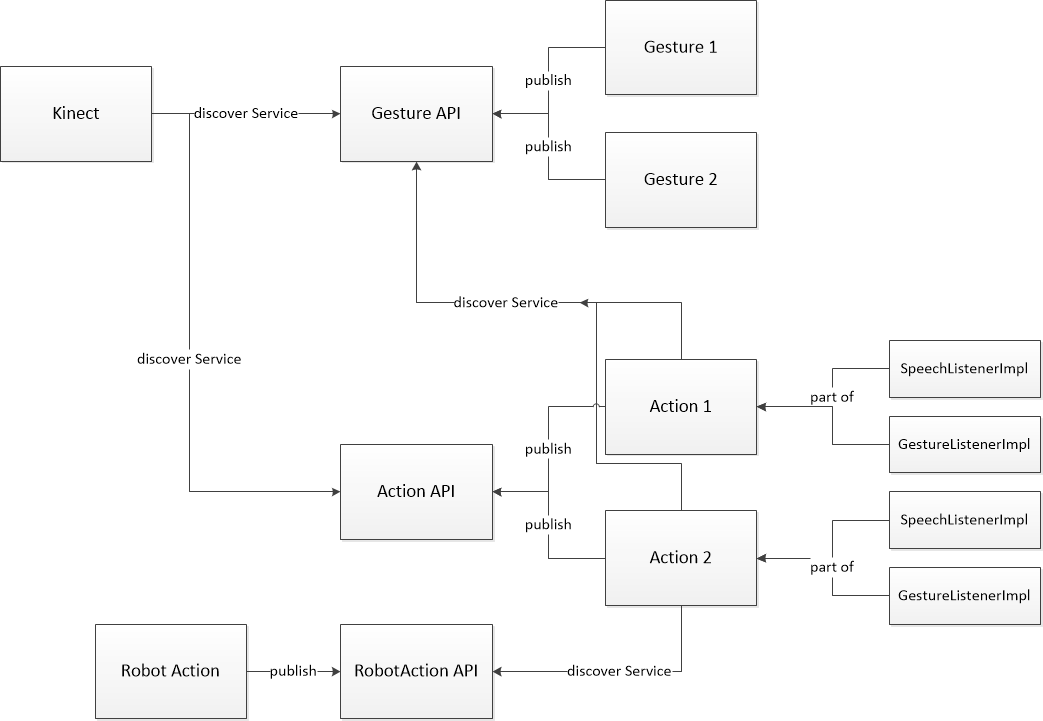
\includegraphics[width=1\textwidth]{img/09kapitel/osgi-architecture.png}
\caption[Anwendungsarchitektur]{Architektur der Anwendung}
\label{fig:osgiArchitecture}
\end{figure}

\section{Bundles}
\label{sec:osgiBundles}

Bundles stellen ihre Funktionalit\"at mittels Services zur Verf\"ugung. Dies geschieht mittels eines Interface. 
Das Interface wird in einem eigenen Bundle definiert. Hierdurch entsteht eine statische Abh\"angigkeit 
zwischen einem API-Bundle und seinen implementierenden Bundles. Dieser wird geschaffen mittels der Deklaration von importierten 
und exportierten Bundles im Manifest des Bundles (Abbildung~\ref{listing:manifestGestureAPI}). Die OSGi-Runtime liest beim Start 
eines Bundles das Manifest ein und l\"ost die Abh\"angigkeiten auf. Ist dies nicht m\"oglich, kann ein Bundle nicht gestartet werden. 
Ebenso k\"onnen laufende Bundles wieder beendet werden. Hierf\"ur existiert das Konzept des Bundle-Lifecycle~\footnotemark[3].

\newpage
\par\smallskip
\lstset{language=Java}
\begin{lstlisting}[caption={Manifest der Gesture API}, label={listing:manifestGestureAPI}]
Manifest-Version: 1.0
Bundle-ManifestVersion: 2
Bundle-Name: Rocovomo Gesture API
Bundle-SymbolicName: de.rocovomo.jnect.gesture
Bundle-Version: 0.0.1.qualifier
Bundle-RequiredExecutionEnvironment: JavaSE-1.7
Import-Package: org.eclipse.emf.common,
 org.eclipse.emf.ecore,
 org.jnect.gesture
Export-Package: de.rocovomo.jnect.gesture.api,
 de.rocovomo.jnect.gesture.provider.api
\end{lstlisting}
\par\smallskip

\subsection{Kinect}

<<<<<<< HEAD
Das Kinect-Bundle hat Abh\"angigkeiten zu den jnect-Bundles. In dieser Komponente wird die Anbindung zur Kinect implementiert. Dieses Bundle 
sucht nach Services, welche durch die Gesture- und Action-Bundles zur Verf\"ugung gestellt werden. Es registriert Gesten, sowie die 
Gesten-Listener und Sprach-Listener der Action-Bundles an der Kinect. Durch die Listener erhalten die Action-Bundles die Information 
ob sie ausgel\"ost wurden. Das Bundle stellt die effiziente Verwaltung von Gesten und Listenern sicher, sowie die Verwaltung der 
angeschlossenen Kinect. Ohne das Kinect for Windows \acrshort{SDK} kann dieses Bundle nicht gestartet werden.

\subsection{Gesture}

In den Gesture-Bundles werden Gesten implementiert. Finden Ver\"anderungen im Modell statt, so wird dies den Gesture-Bundles mitgeteilt und 
diese analysieren mittels HMMs ob sie ausgel\"ost wurden. Gesten stellen sich als Service zur Verf\"ugung. Sie werden vom Kinect-Bundle zur 
Erkennung verwendet. Auch die Action-Bundles m\"ussen ihre entsprechenden Gesten kennen. Gesten werden als unabh\"angige Bundles von Aktionen 
realisiert. Hierdurch wird eine Codeduplikation bei Aktionen die gleiche Gesten verwenden vermieden.

Die Implementierung einer Geste muss von der jnect-Klasse \textit{Gesture}~(Listing \ref{listing:Gesture}) erben. In der Methode 
\textit{isGestureDetected(\ldots)} wir das HMM zur Erkennung der Geste implementiert. Ist die Gesten am Gesten-Proxy der Kinect 
angemeldet, so wird der \textit{GestureListener}, welcher diese Geste nutzt aufgerufen.

\par\smallskip
\lstset{language=Java}
=======
\section{Architektur}

Nachfolgend wird der derzeitige Stand der Architektur der Anwendung beschrieben. Da dies lediglich der erste Teil einer gr\"oßeren Arbeit ist, k\"onnen infolge des zweiten Teils der Arbeit Ver\"anderungen an der Architektur auftreten. 

Wie in Abschnitt~\ref{subsec:OSGi} bereits angesprochen, wird die Anwendung unter Verwendung von OSGi~\footnotemark[1] umgesetzt. Als Implementierung des OSGi-Standard wurde im Rahmen dieser Arbeit das Framework Equinox~\footnotemark[2] gew\"ahlt. Die Eclipse IDE und die von jnect verwendeten Frameworks basieren ebenfalls auf dieser Plattform, sie ist daher optimal geeignet. Durch Implementierung der Gesten, Sprachbefehle und Aktionen durch OSGi-Bundles~\footnotemark[3] ist es m\"oglich zur Laufzeit der Anwendung neue Gesten nachzuladen oder Aktionen neu zu definieren. Geschaffen wird diese lose Kopplung der Komponenten durch die Nutzun der Service-Funktionalit\"at der OSGi-Plattform.

In Abbildung~\ref{fig:osgiArchitecture} ist die aktuelle Architektur der Anwendung zu sehen. In Abschnitt~\ref{sec:osgiBundles} werden die dargestellten Komponenten n\"aher beschrieben. Die Komponenten stellen ihre Funktionalit\"at in Form von Services~\footnotemark[3] bereit. Ein Service wird mittels eines Interface am Framework registriert. Somit k\"onnen andere Bundles einen Service nutzen, ohne dessen konkrete Implementierung 
kennen zu m\"ussen.

\footnotetext[1]{Osgi Alliance (2013) \href{http://www.osgi.org/Technology/HomePage}{\textit{OSGi Alliance}} osgi.org, Abgerufen Januar 07, 2013}
\footnotetext[2]{The Eclipse Foundation (2013) \href{http://www.eclipse.org/equinox/}{\textit{Eclipse Equinox}} eclipse.org, Abgerufen Januar 07, 2013}
\footnotetext[3]{Osgi Alliance (2013) \href{hhttp://www.osgi.org/Technology/WhatIsOSGi}{\textit{OSGi Technology}} osgi.org, Abgerufen Januar 07, 2013}

\begin{figure}[htb]
\centering
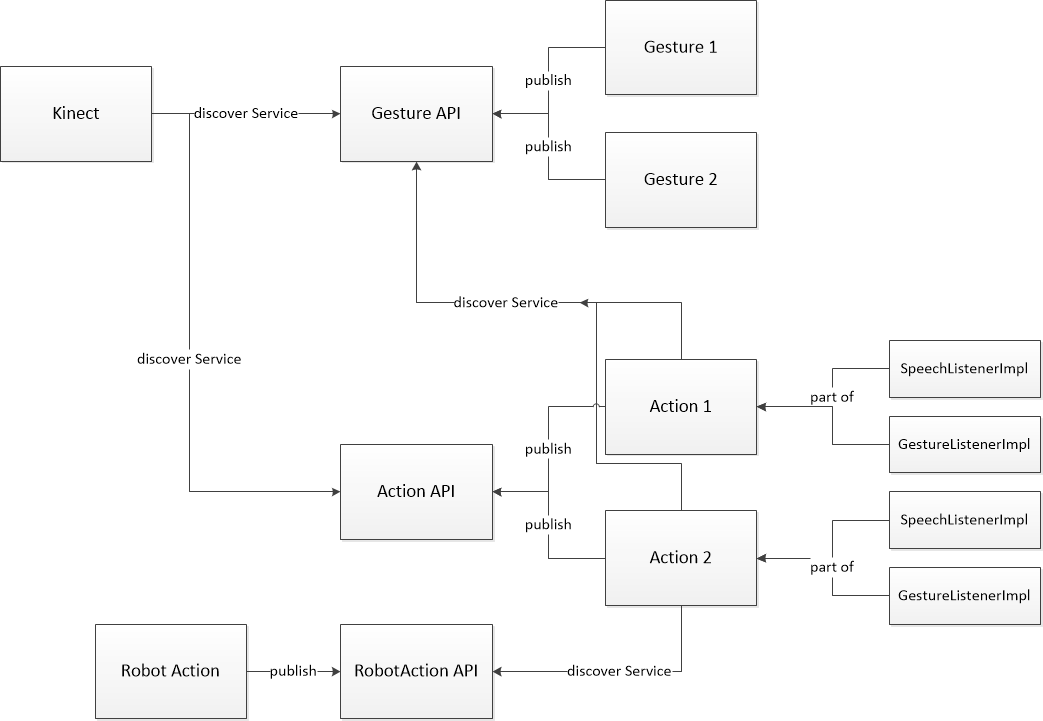
\includegraphics[width=1\textwidth]{img/09kapitel/osgi-architecture.png}
\caption[Anwendungsarchitektur]{Architektur der Anwendung}
\label{fig:osgiArchitecture}
\end{figure}

\section{Bundles}
\label{sec:osgiBundles}

Bundles stellen ihre Funktionalit\"at mittels Services zur Verf\"ugung. Dies geschieht mittels eines Interface. Das Interface wird in einem eigenen Bundle definiert. Hierdurch entsteht eine statische Abh\"angigkeit zwischen einem API-Bundle und seinen implementierenden Bundles. Dieser wird geschaffen mittels der Deklaration von importierten und exportierten Bundles im Manifest des Bundles (Abbildung~\ref{listing:manifestGestureAPI}). Die OSGi-Runtime liest beim Start eines Bundles das Manifest ein und l\"ost die Abh\"angigkeiten auf. Ist dies nicht m\"oglich, kann ein Bundle nicht gestartet werden. Ebenso k\"onnen laufende Bundles wieder beendet werden. Hierf\"ur existiert das Konzept des Bundle-Lifecycle~\footnotemark[3].

\lstset{language=Java,
 basicstyle=\footnotesize, 
 numbers=left,
 captionpos=b,
 showspaces=false,             
 showstringspaces=false,}
\begin{lstlisting}[caption={Manifest der Gesture API}, label={listing:manifestGestureAPI}]
Manifest-Version: 1.0
Bundle-ManifestVersion: 2
Bundle-Name: Rocovomo Gesture API
Bundle-SymbolicName: de.rocovomo.jnect.gesture
Bundle-Version: 0.0.1.qualifier
Bundle-RequiredExecutionEnvironment: JavaSE-1.7
Import-Package: org.eclipse.emf.common,
 org.eclipse.emf.ecore,
 org.jnect.gesture
Export-Package: de.rocovomo.jnect.gesture.api,
 de.rocovomo.jnect.gesture.provider.api
\end{lstlisting}

\subsection{Kinect}

Das Kinect-Bundle hat Abh\"angigkeiten zu den jnect-Bundles. In dieser Komponente wird die Anbindung zur Kinect implementiert. Dieses Bundle sucht nach Services, welche durch die Gesture- und Action-Bundles zur Verf\"ugung gestellt werden. Es registriert Gesten, sowie die Gesten-Listener und Sprach-Listener der Action-Bundles an der Kinect. Durch die Listener erhalten die Action-Bundles die Information ob sie ausgel\"ost wurden.
Das Bundle stellt die effiziente Verwaltung von Gesten und Listenern sicher, sowie die Verwaltung der angeschlossenen Kinect. Ohne das Kinect for Windows SDK kann dieses Bundle nicht gestartet werden.

\subsection{Gesture}

In den Gesture-Bundles werden Gesten implementiert. Finden Ver\"anderungen im Modell statt, so wird dies den Gesture-Bundles mitgeteilt und diese analysieren mittels HMMs ob sie ausgel\"ost wurden. Gesten stellen sich als Service zur Verf\"ugung. Sie werden vom KinectBundle zur Erkennung verwendet. Auch die Action-Bundles m\"ussen ihre entsprechenden Gesten kennen. Gesten werden als unabh\"angige Bundles von Aktionen realisiert. Hierdurch wird eine Codeduplikation bei Aktionen die gleiche Gesten verwenden vermieden.

\lstset{language=Java,
 basicstyle=\footnotesize, 
 numbers=left,
 captionpos=b,
 showspaces=false,             
 showstringspaces=false,}
>>>>>>> 2bb7e10335176dc446d28fa0516733abbf1cc9ef
\begin{lstlisting}[caption={Klasse Gesture}, label={listing:Gesture}]
public abstract class Gesture extends EContentAdapter {

	private GestureProxyCallback gestureProxy;

	/**
	 * DO NOT CALL THIS METHOD, IT WILL BE CALLED BY THE GESTUREPROXY
	 * 
	 * @param gestureProxy
	 *            the proxy to notify when a gesture is detected
	 */
	public void setGestureProxy(GestureProxyCallback gestureProxy) {
		this.gestureProxy = gestureProxy;
	}

	@Override
	public void notifyChanged(Notification notification) {
		if (gestureProxy != null && isGestureDetected(notification)) {
			this.gestureProxy.notifyGestureDetected(this.getClass());
		}
	}

	/**
	 * checks whether the searched gesture is detected
	 * 
	 * @param notification
	 *            the notification containing the model changes
	 * @return true if the gesture was detected
	 */
	protected abstract boolean isGestureDetected(Notification notification);
}
\end{lstlisting}
<<<<<<< HEAD
\par\smallskip

\subsection{Action}
\label{subsec:osgiaction}

Die Action-Bundles bilden einen Befehl ab. Dieser Befehl kann entweder eine Geste, ein Sprachbefehl oder eine Kombination aus beidem sein. 
Je nachdem verf\"ugt die Action \"uber einen \textit{Speech}- oder einen \textit{GestureListener}. Eine Kombination aus beidem ist hier 
auch m\"oglich. Die Integration dieser beiden Eingabeoptionen wird von Buxton~\cite{bib:buxton}~\footnotemark[4] in Form von Frames besprochen. 
Eine Aktion ist abh\"angig von einer Geste die von einem Gesture-Bundle bereitgestellt wird.

Wird eine Geste erkannt wird die Methode \textit{notifyGestureDectected(\ldots)} der entsprechenden Implementierung der abstrakten Klasse
\textit{GestureListener} (Listing~\ref{listing:GestureListener}) aufgerufen. Von hier kann dann die entsprechende Roboter-Aktion aufgerufen werden.

Das Vorgehen ist beim \textit{SpeechListener}~(\ref{listing:SpeechListener}) prinzipiell \"ahnlich. Wird ein Sprach-String der Implementierung
des \textit{SpeechListener} erkannt, so wird die entsprechende Methode, \textit{notifySpeech(\ldots)} aufgerufen. Im Gegensatz zur Geste ist die
Sprache weniger komplex und wird nur mittels Strings definiert. Diese erh\"alt der \textit{KinectManager} mittels \textit{getWords(\ldots)}.

Bislang stellt sich das Action-Bundle selbst als Service zur Verf\"ugung. Das Kinect-Bundle erh\"alt so Zugriff auf die \textit{Speech-} und 
\textit{GestureListener}.

\footnotetext[4]{Kapitel 14 Multimodal Integration}

\par\smallskip
\lstset{language=Java}
=======

\subsection{Action}

Die Action-Bundles bilden einen Befehl ab. Dieser Befehl kann entweder eine Geste, eine Sprachbefehl oder eine Kombination aus beidem sein. Je nachdem verf\"ugt die Action \"uber einen Speech- oder einen GestureListener. Eine Kombination aus beidem ist hier auch m\"oglich. Eine Aktion ist abh\"angig von

\lstset{language=Java,
 basicstyle=\footnotesize, 
 numbers=left,
 captionpos=b,
 showspaces=false,             
 showstringspaces=false,}
>>>>>>> 2bb7e10335176dc446d28fa0516733abbf1cc9ef
\begin{lstlisting}[caption={Klasse GestureListener}, label={listing:GestureListener}]
public abstract class GestureListener {

	/**
	 * callback method, that gets called when a {@link Gesture} is detected
	 * 
	 * @param gesture
	 *            - the class of the {@link Gesture} that was detected
	 */
	public abstract void notifyGestureDetected(Class<? extends Gesture> gesture);

	/**
	 * {@link Set} of {@link Gesture}s this {@link GestureListener} listens to
	 * 
	 * @return {@link Set} of {@link Gesture}s to be notified about, can be
	 *         empty but not null
	 */
	public Set<Gesture> getGestures() {
		return Collections.emptySet();
	}

	/**
	 * Whether the {@link GestureListener} listens only to special
	 * {@link Gesture}s.
	 * 
	 * @return true if only the {@link Gesture}s provided in
	 *         {@link #getGestures()} should be provided to the listener, false
	 *         otherwise
	 */
	public boolean isFiltered() {
		return false;
	}
\end{lstlisting}
<<<<<<< HEAD
\par\smallskip

\par\smallskip
\lstset{language=Java}
=======

\lstset{language=Java,
 basicstyle=\footnotesize, 
 numbers=left,
 captionpos=b,
 showspaces=false,             
 showstringspaces=false,}
>>>>>>> 2bb7e10335176dc446d28fa0516733abbf1cc9ef
\begin{lstlisting}[caption={Klasse SpeechListener}, label={listing:SpeechListener}]
public abstract class SpeechListener {
	/**
	 * callback when a relevant speech is recognized
	 * 
	 * @param speech
	 *            - the speech recognized
	 */
	public abstract void notifySpeech(String speech);

	/**
	 * a set of words that this {@link SpeechListener} wants to be recognized
	 * and notified about
	 * 
	 * @return a {@link Set} of {@link String}s building the relevant words
	 */
	public abstract Set<String> getWords();

	/**
	 * if a {@link SpeechListener} is filtered than it will be only notified
	 * about recognized words that are contained in the {@link Set} provided by
	 * {@link #getWords()}
	 * 
	 * @return true if should be filtered, false otherwise
	 */
	public boolean isFiltered() {
		return true;
	}
}
\end{lstlisting}
<<<<<<< HEAD
\par\smallskip

\subsection{Robot Action}
\label{subsec:Roboterschnittstelle}

Bundles, welche die Robot Action \acrshort{API} implementieren, stellen sich ebenfalls als Services zur Verf\"ugung. Action-Bundles stellen auf dieser 
Basis eine Verbindung zwischen Geste/Sprachbefehl und Roboter-Aktion her. Grunds\"atzlich k\"onnte man dies auch umgekehrt konstruieren, dass
sich die Roboter-Aktion ein passendes Action-Bundle sucht. Da Roboter-Interaktion Teil des zweiten Teils der Arbeit ist, ist dieses Bundle 
bisher noch ohne jede Funktionalit\"at.

\section{User Interface}

Als User-Interface ist eine Anwendung auf Basis der \gls{RCP} von Eclipse vorgesehen. Zur Visualisierung der 
der Eingaben des Nutzers war eine dreidimensionale Umgebung mit Hilfe der \gls{LWJGL} vorgesehen. 
Optisch orientiert sich eine Anwendung auf dieser Plattform am Aussehen der Eclipse IDE, zu sehen in Abbildung~\ref{fig:eclipse}. 
Bislang kann das Skeleton-Modell in einem GEF-Editor dargestellt werden, dies wurde in Abbildung~\ref{fig:gef} bereits gezeigt. Erkannte Gesten und Sprachbefehle werden bislang auf einer Logging-Konsole
ausgegeben.

\begin{figure}[htb]
\centering
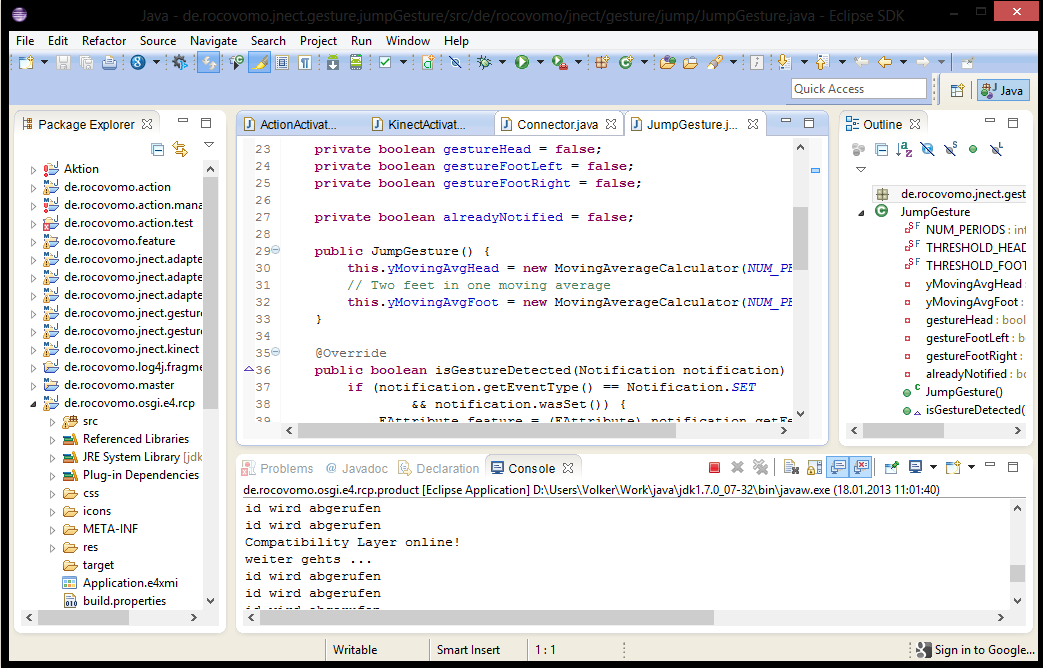
\includegraphics[width=1\textwidth]{img/09kapitel/rcp.png}
\caption[Eclipse IDE]{Eclipse IDE}
\label{fig:eclipse}b
\end{figure}

=======

\subsection{Robot Action}

\section{User Interface}

>>>>>>> 2bb7e10335176dc446d28fa0516733abbf1cc9ef

	\chapter{Ausblick - weitere Arbeiten}
\label{chap:Ausblick}

Mit dieser Arbeit wurden die n\"oetigen Grundlagen geschaffen auf deren Basis in der nachfolgenden Arbeit die Ansteuerung 
eines mobilen Roboters erfolgen kann. Mit Hilfe der entwickelten Anwendung ist es m\"oglich erste Gesten und Sprachkommandos zu erfassen und die Schnittstellen
% The End
	
% Abbildungsverzeichnis
	\cleardoublepage
	\phantomsection \label{listoffig}
	\addcontentsline{toc}{chapter}{Abbildungsverzeichnis}
	\listoffigures

% Tabellenverzeichnis
	\cleardoublepage
	\phantomsection \label{listoftab}
	\addcontentsline{toc}{chapter}{Tabellenverzeichnis}
	\listoftables

% Quellcodeverzeichnis
	\cleardoublepage
	\phantomsection \label{listoflist}
	\renewcommand\lstlistlistingname{Quellcodeverzeichnis}
	\addcontentsline{toc}{chapter}{Quellcodeverzeichnis}
	\lstlistoflistings
	
% Bibliography:
	\cleardoublepage
	\phantomsection \label{listoflit}
	\renewcommand{\bibname}{Literaturverzeichnis}
	\addcontentsline{toc}{chapter}{Literaturverzeichnis}
	\bibliographystyle{alpha}
	\bibliography{bib}

% Glossary
	% Acronyms
	\printglossary[type=\acronymtype]
	
	% Glossary
	\printglossary[style=altlist,title=Glossar]

% Appendix
	%\appendix
	%\input{content/appendicies/01appendix}
	%\input{content/appendicies/02appendix}
	%\input{content/appendicies/03appendix}
\end{document}